%%%%%%%%%%%%%%%%%%%%%%%%%%%%%%%%%%%%%%%%%%%%%%%%
%%%%%%%%%%%%%Przykładowy dokument%%%%%%%%%%%%%%%
%%%%%%%%%%wraz z klasą pracadyp.cls%%%%%%%%%%%%%
%%%%%%%%%%%%%%%%%%%%%%%%%%%%%%%%%%%%%%%%%%%%%%%%

% w nawiasie kwadratowym wpisujemy rodzaj pracy: 
% magisterska, licencjacka, inzynierska
\documentclass[licencjacka]{pracadypl}


%% ważne definicje %%
\usepackage{tgtermes}
\usepackage[T1]{fontenc}
\usepackage{polski}
\usepackage[utf8]{inputenc}
\input glyphtounicode
\pdfgentounicode=1
\usepackage{amssymb}
\usepackage{amsmath}
\usepackage{graphicx}
\usepackage{titlesec}
\usepackage{color}
\usepackage{xcolor}
\usepackage{float}
\usepackage{tablefootnote}
\usepackage{hyperref}
\usepackage{titling}
\usepackage{interval}
\bibliographystyle{plain}

\def\mgr{magisterska}
\def\lic{licencjacka}
\def\inz{inżynierska}

\def\sk{Słowa kluczowe}
\def\kw{Keywords}
\def\et{Title in English}
%% koniec ważnych definicji %%



%% wypełnia Autor pracy %%

%autor pracy
\author{Kajetan Owczarek}
%numer albumu
\nralbumu{396396}
%tytuł pracy
\title{Przykłady zastosowania technik optymalizacji czasu wczytywania witryny internetowej}
%kierunek studiów
\kierunek{Informatyka}
%promotor w dopełniaczu
\opiekun{prof. dr Wojciecha Horzelskiego}
\katedra{Katedra Informatyki Stosowanej}
%rok
\date{2023}
%Słowa kluczowe:
\slkluczowe{pierwsze, drugie, trzecie, czwarte}
%tytuł po angielsku
\tytulang{Title in English}
%słowa kluczowe po angielsku
\keywords{first, second, third, fourth}
%% koniec ważnych definicji %%

%% APD %%
%% w systemie APD należy jeszcze wpisać, poza powyższymi informacjami, streszczenie oraz streszczenie w języku angielskim  %%


%%% definicje %%%
\def\pd{\noindent \textbf{Dowód.~}} %%początek dowodu
\def\kd{\hfill\mbox{$\rule{2mm}{2mm}$}} %%koniec dowodu
\newtheorem{defi}{Definicja}[section]
\newtheorem{uwaga}{Uwaga}[section]
\newtheorem{tw}{Twierdzenie}[section]
\newtheorem{lem}{Lemat}[section]
\newtheorem{wn}{Wniosek}[section]
\renewcommand\thetw{\thesection.\arabic{tw}.}
\renewcommand\thedefi{\thesection.\arabic{defi}.}
\renewcommand\theuwaga{\thesection.\arabic{uwaga}.}
\renewcommand\thetw{\thesection.\arabic{tw}.}
\renewcommand\thelem{\thesection.\arabic{lem}.}
\renewcommand\thewn{\thesection.\arabic{wn}.}
%
\definecolor{wmiigreen}{rgb}{0.0, 0.5, 0.0}
\titleformat{\chapter}[display]
  {\normalfont\huge\bfseries\color{wmiigreen}}{\chaptertitlename\ \thechapter}{10pt}{\Huge}
 %
\linespread{1.3}
%%% koniec definicji ze wzorca %%%


%%% osobiste definicje

\newcommand{\selfnote}[1]{\colorbox{pink}{#1}}
\hypersetup{
  colorlinks=false,
  linkcolor=red,
  pdftitle={\thetitle},
  pdfborder={0 0 0}
}
\intervalconfig{
  soft open fences
}

%%% koniec definicji

\begin{document}

\maketitle
\tableofcontents
\newpage



\chapter{Wstęp}

Pomimo nieustającego rozwoju technologii telekomunikacyjnych oraz zwiększania prędkości łączy internetowych, problem wydajności usług internetowych nie zniknął, ani nie zapowiada się, aby tak się zadziało w n. Od potrzeb łączności poza terenami zabudowanymi, przez starzejący lub ograniczony sprzęt, po malejącą cierpliwość użytkowników, dostarczanie treści z serwera do urządzenia użytkownika szybko i efektywnie jest jednym z głównych celów w pracy ze stronami internetowymi.

Celem tej pracy jest zaprezentowanie serii technik i optymalizacji, pozwalających na poprawienie czasów wczytywania witryn internetowych na urządzeniach użytkownika, oraz porównanie ich przy pomocy obiektywnych i powszechnie stosowanych narzędzi i metryk.

Celem zilustrowania efektów takich optymalizacji, a dokładniej wpływ ich braku na używalność strony, stworzono przykładową stronę, zrobioną przy użyciu najprostszych, najpopularniejszych technik. Ma ona reprezentować witrynę, która zrobiona jest kompetentnie, acz z minimalną uwagą przyłożoną do wydajności strony pod względem procesów wczytywania i uruchamiania strony. Następnie, poprzez stosowanie technik wpływających minimalnie na funkcjonalność strony, poprawione zostaną wyniki pomiarów obiektywnych.

\section{Sposób pomiarów}
Celem usunięcia jak najwięcej zewnętrznych zmiennych w danych pomiarowych,
% \footnote{Choć dla porównania wydajności wyniki z jednej maszyny powinny wystarczyć, niestety zaobserwowałem znaczne, trudne do zrozumienia fluktuacje wydajności mojego komputera. Wyniki na nim były by więc wewnętrznie niespójne.}
skorzystano z narzędzia \texttt{WebPageTest}.

\texttt{WebPageTest} to operowana przez firmę Catchpoint usługa, pozwalająca na wykonanie dokładnego pomiaru wczytywania strony w wybranym regionie, na emulowanym urządzeniu, w określonych warunkach sieciowych. Używając standaryzowanego środowiska, można usunąć wiele zmiennych wynikających z aktywności innych aplikacji na testującej maszynie oraz innych urządzeń w sieci. Sprawia to też, że wyniki są o wiele bardziej uniwersalne - mogąc odnieść się do środowiska ze znanymi charakterystykami wydajności, redukowany jest element niepewności i zgadywania, jak sposób testowania wpłynął na otrzymane pomiary. 

\texttt{WebPageTest} dostarcza dokładny zapis procesu wczytywanie testowanej witryny. Dane te są prezentowane w formie złożonego wykresu, o którym zostanie opowiedziane więcej w późniejszym rozdziale.

% Rozważałem wcześniej użycie do pomiarów stworzonego przez Google narzędzia o nazwie Lighthouse, które stara się spełnić podobną funkcję oceny wydajności, acz analizuje też wiele innych metryk dotyczączych rzeczy jak używanie technologii pomagających osobą używającym czytników ekranu, optymalizacji pod kątem wyszukiwarek internetowych, czy współczesności strony. Niestety, sposób działania Lighthouse'a jest ograniczony w swojej dokładności. Zamiast dokonywać pełnej symulacji wydajności standardowego urządzenia, dokonuje on testy w pełnej prędkości, a następnie przeskalowując je. Tak jak nie jest to zła metoda żeby optymalizować lokalnie, gdyż Lighthouse sugeruje też sposoby poprawy, tak użycie go nie eliminuje częściowej zmienności wynikających z natury maszyny, na którym są dokonywane pomiary.

\section{Startowy projekt}
Żeby zilustrować techniki, które zostaną omówione później, oraz ich wpływ na wydajność wczytywania strony, potrzebna jest na to przestrzeń w formie przykładowej witryny. Celem podczas tworzenia jej było zawarcie łatwych do popełnienia błędów oraz podjęcie decyzji niesprzyjających czasowi wczytywania. Stworzono więc udawaną stronę z wiadomościami. Zawiera ona paręnaście zdjęć, dużo tekstu, oraz dwa elementy interaktywne. 

\begin{figure}[H]
  
\includegraphics[width=\linewidth]{images/frontpage.png}
  \caption{Nagłówek strony oraz karuzela z wiadomościami, czyli jeden z elementów interaktywnych. Przewijają się na niej trzy elementy zawierające zdjęcia, tytuły i wstępy artykułów.}
  \label{fig:frontpage}
\end{figure}

\begin{figure}[H]
  
\includegraphics[width=\linewidth]{images/frontpage-articles.png}
  \caption{Fragment listy artykułów, która zawiera te same elementy co ww. karuzela, lecz w innym, nieinteraktywnym formacie.}
  \label{fig:frontpage-articles}
\end{figure}

\begin{figure}[H]
  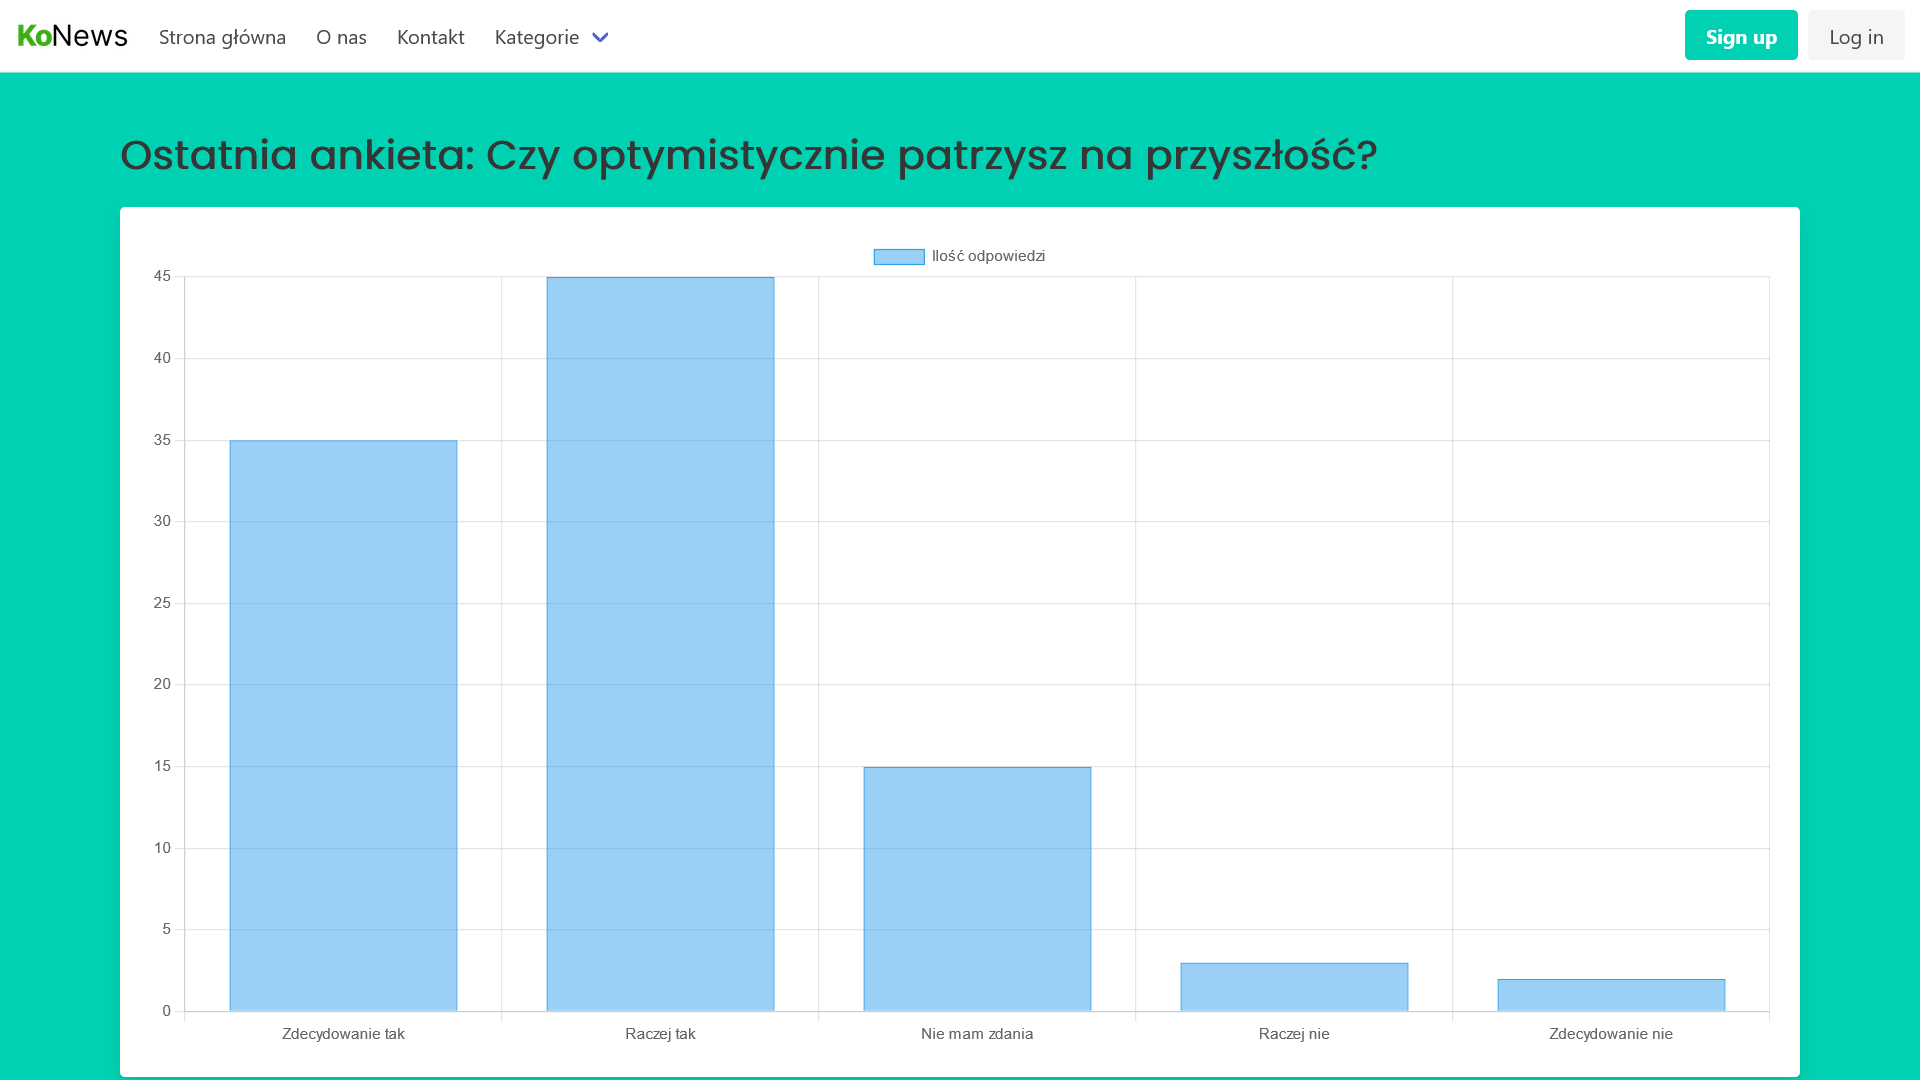
\includegraphics[width=\linewidth]{images/frontpage-dynamic-article.png}
  \caption{Interaktywna prezentacja wyników ankiety, wczytująca dane z serwera, i wyświetlające je w formie wykresu, wzbogaconego animowanymi zmianami elementów przy najechaniu na nie.}
  \label{fig:frontpage-dynamic}
\end{figure}

Żeby zaprezentować efekty dużej ilości treści w dokumencie \texttt{HTML}, dodano do niej jedno ze źródeł do treści tu zawartej, czyli specyfikację parsowania dokumentów \texttt{HTML}.

\begin{figure}[H]
  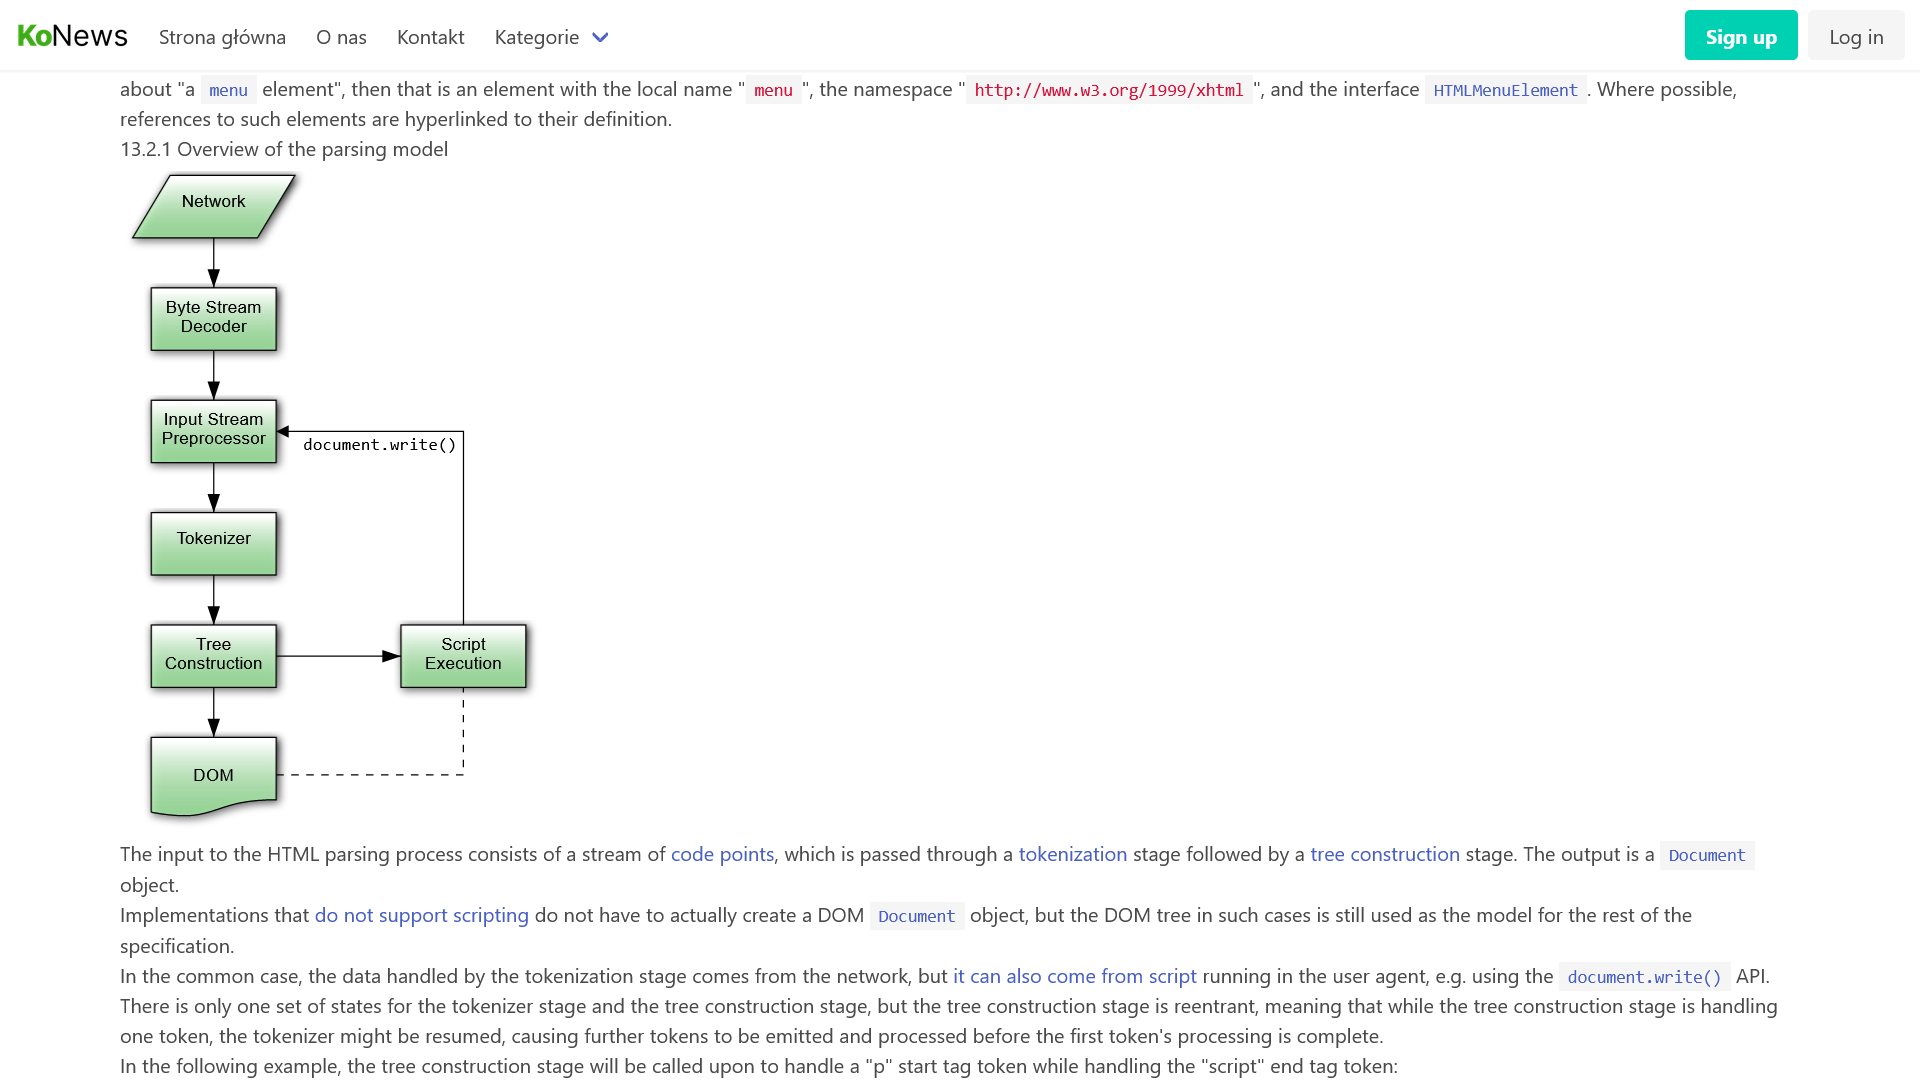
\includegraphics[width=\linewidth]{images/frontpage-spec.png}
  \caption{Specyfikacja parsowania \texttt{HTML}, załączona pod koniec witryny}
  \label{fig:frontpage-spec}
\end{figure}




\section{Wstępna analiza wydajności}
Przed rozpoczęciem optymalizacji witryny, należy zbadać, jak zachowuje się ona przed zminami. Optymalizując na ślepo, jest prosto zmarnować czas na optymalizacjach, które nie zmieniają finalnej wydajności. W przypadku tworzenia witryn internetowych jest to szczególnie prosty do popełnienia błąd. Interakcja równoległego wczytywania zasobów, oraz mechanizm zasobów blokujących może sprawić, że dowolne przyśpieszenie jednej części nie wpłynie zupełnie na finalną szybkość wczytania, gdyż dalsze kroki nie mogą być rozpoczęte przed pełnym ukończeniem wszystkich wcześniejszych.

Głównym wynikiem wykonywania analiz przy pomocy \texttt{WebPageTest}'u jest wykres zwany waterfall'em, czyli wodospadem. Jest on bardzo gęsty w dane i zawiera przede wszystkim dane o połączeniach sieciowych oraz stanie przeglądarki. Omówione zostaną podstawy odczytywania takiego\footnote{Dostepna na stronie \texttt{WebPageTest}'u lekko interaktywna wersja tego wykresu pozwala odczytać te dane nieco prościej, oraz daje dostęp do dodatkowych informacji, których nie ma na obrazkowym waterfall'u.}, równocześnie zwracając uwagę na problemy, które można zobaczyć ze wstępnych testów.
\begin{figure}[h!]
  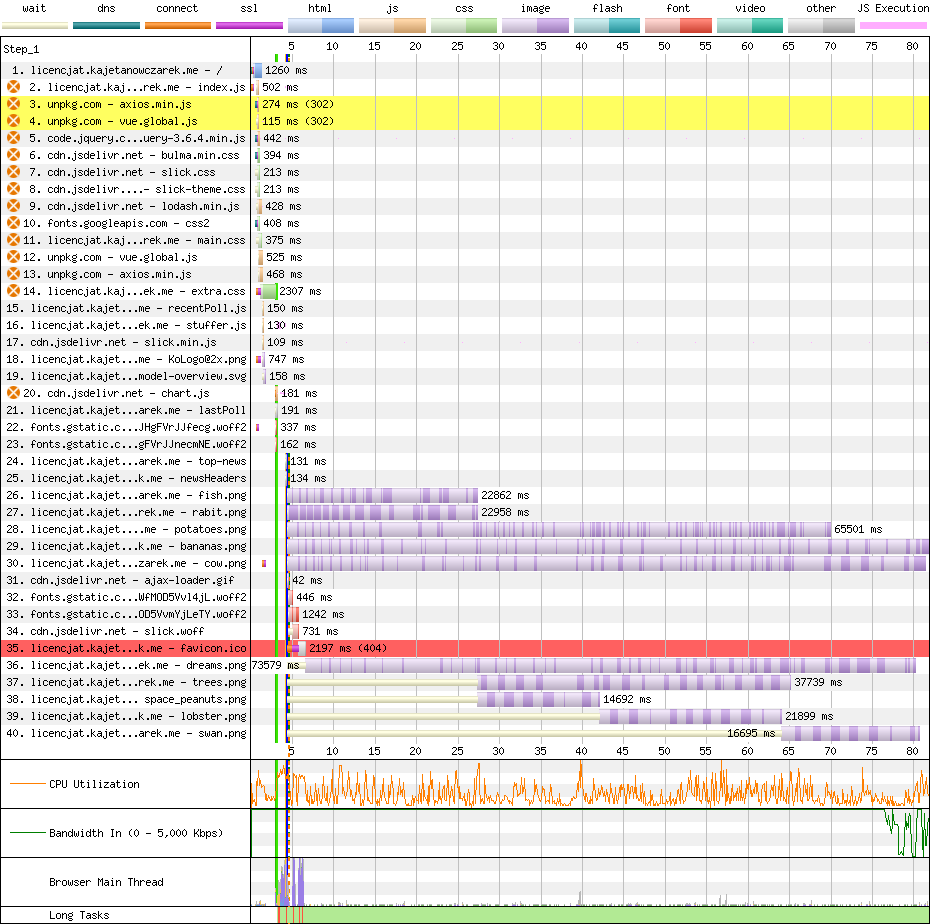
\includegraphics[width=\linewidth]{images/base-waterfall-all-final.png}
  \caption{Wykres produkowany przez \texttt{WebPageTest}, zwany jako Waterfall}
  \label{fig:waterfall-base}
\end{figure}
Na górze wykresu znajduje się legenda, informująca użytkownika, które kolory na wykresie oznaczają jaką fazę rozpoczynania połączeń, oraz rodzaje treści przez te połączenia przesyłane. 

Tuż pod nią, znajduje się główna część, która zawiera najważniejsze dane, czyli wykres rozkładu czasowego realizacji kolejnych zapytań wykonywanych przez przeglądarkę. Od góry do dołu znajdują się kolejne zapytania \texttt{HTTP}, od rozpoczętego najwcześniej do najpóźniej. Od lewej do prawej zaznaczony jest upływ czasu. Same okresy, kiedy zapytania witryny były realizowane, są zaznaczone jako prostokąty na wykresie. Poprzez cienkie prostokąty są zaznaczane obszary czasu, kiedy połączenia nie postępowały stan wczytania naszej strony, specyficznie otwieranie połączeń i wykonywanie kodu JavaScript. Grubymi prostokątami jest zaznaczone, kiedy połączenia było otwarte i gotowe na transfer danych, na blado kiedy nie są przesyłane dane, oraz na mocniejszy kolor kiedy są.

Poniżej głównego wykresu znajdują się wykresy zawierające informacje o wykorzystaniu procesora. W sytuacji, gdzie gotowość strony powstrzymuje ilość danych, które są w procesie wczytywania przetwarzane, to ten wykres będzie pokazywał, że tak się dzieje.

Jeszcze niżej, znajduje się wykres zużycia łącza. Im linia na nim jest wyżej, tym więcej dostępnego dla testowego urządzenia łącza jest wykorzystywane. W większości sytuacji pożądane jest, aby liczba ta była jak najwyższa, gdyż oznacza to, że wczytywanie jest ograniczane przez zewnętrzne warunki sieciowe, a nie specyfikacja urządzenia lub działanie kodu witryny.

Przedostatni wiersz jest zajęty przez wykres przetwarzania wykonywanego przez przeglądarkę. Wysokością przedstawia on, jak bardzo zajęty jest główny wątek przeglądarki, natomiast kolor sygnalizuje, jakie zużywały najwięcej czasu w danym momencie.

Ostatnim, zarazem najważniejszym i najmniej ważnym, jest wykres interaktywności. Na biało oznaczony jest czas, zanim strona była użytkownikowi wyświetlona, na czerwono kiedy przeglądarka była zbyt zajęta, by reagować na wejścia, a na zielono, kiedy wszystko działało. Tak jak wykres ten ilustruje bardzo ważny aspekt działania strony - dominacja czerwieni oznacza, że dla użytkownika wszystko wydaje się zacięte - tak nie daje on informacji, czemu tak się dzieje, oraz sugestii, co można zmienić. Na szczęście wykres tuż nad nim bardzo silnie przekłada się na interaktywność, więc można traktować je jako wspólną część, górny jako dokładną wartość, dolny jako miarkę, czy przekroczyliśmy punkt upadku używalności. 

Prócz tego, przez cały wykres przebiega kilka pionowych linii, które oznaczają kluczowe momenty we wczytywaniu strony. Są nimi momenty, kiedy użytkownikowi wyświetliło się na ekranie cokolwiek (ang. \emph{First Contentful Paint}, \texttt{FCP}), kiedy strona mogła po raz pierwszy reagować na wejścia użytkownika (ang. \emph{Time To Interactive}, \texttt{TTI}), czy kiedy nastąpiła największa zmiana wyglądu (ang. \emph{Largest Contentful Paint}, \texttt{LCP}). Na tej wersji wykresu nie widać ich zbyt dobrze, gdyż wszystkie oznaczane tak wydarzenia zdarzyły się względnie wcześnie. Jednakże, na późniejszych wersjach wykresów, będzie można użyć ich, żeby znaleźć najważniejsze dla odczucia strony punkty w procesie ładowania witryny.

Wiedząc, co oznaczają części waterfall'a, można zauważyć, że wczytywanie strony dominuje parę fioletowych zapytań. Korzystając z legendy i zrozumienia, jak wykres ten czytać, można wywnioskować, że są to zdjęcia, które wczytują się długo i walczą o użycie łącza, spędzając większość czasu w oczekiwaniu na wolne łącze. Tak samo patrząc na wykres przepustowości łącza widać, że całość przydzielonego urządzeniu łącza jest wykorzystywana przez większość czasu wczytywania strony. Nie jest to zła rzecz, gdyż oznacza to, że strona może wczytywać się szybciej, o ile tylko dostanie szybsze połączenie.

\chapter{Optymalizacja witryny}
\section{Kompresja}
Najprostszym sposobem, aby dodać niesłychaną ilość rozmiaru dowolnemu projektowi komputerowemu, jest użycie nieskompresowanych zasobów w dużej rozdzielczości. Dla przykładu, rozdzielczość FullHD, czyli $1920\times1080\left(=2073600\right)$ pikseli, współcześnie bardzo powszechną w każdej klasie jakościowo-cenowej\footnote{Wg Steam Hardware Survey, ponad 66\% użytkowników platformy Steam posiada właśnie taką rozdzielczość na swoim głównym monitorze. Choć dane tej platformy nie są w pełni reprezentatywne całości populacji użytkowników komputerów, jest to i tak duża ich porcja.}, o standardowej formie zapisu koloru pikseli, czyli 3 kanały po 8 bitów na kanał, daje $2073600\times3\times8 = 49766400$ bitów, czyli $49.77$ megabitów. Mając dostępny przeciętny polski internet, który według statystyk firmy Ookla\footnote{Dane wzięte z \url{https://www.speedtest.net/global-index/poland}} jest w stanie pobrać $107.85$ megabitów na sekundę, pobranie jednego, nieskompresowanego zrzutu ekranu zajęłoby $461$ milisekund. Gdyby więc chcieć po prostu przesłać użytkownikom witryny całość ekranu, który mają widzieć, to bez użycia żadnych optymalizacji przeciętne doświadczenie użytkownika to płynności na poziomie dwóch klatek na sekundę.

Pomimo tego, usługi jak filmy czy seriale online, udostępnianie ekranu na komunikatorach jak Teams czy Discord, lub telekonferecjowanie w dużych grupach z wysokiej jakościami kamerkami jakoś obchodzą ograniczenia prędkości przesyłów i rozmiaru zdjęć i wideo. 
Kluczem do osiągnięcia tej niemożliwości jest kompresowanie przesyłanych danych. Technik na takowe jest wiele, a to która jest najlepsza jest zależne od zawartości transmitowanych informacji. Uniwersalnie, możemy użyć algorytmów bezstratnej kompresji danych, jak \texttt{LZ77} czy kodowanie Huffmana, aby wykorzystać statystyczne właściwości danych, by usunąć niewydajności w zapisie surowych bajtów treści. Dla treści, które na końcu są odbierane przez ludzką percepcję, jak audio czy wideo, możemy często usunąć wiele nieważnych detali. Precyzję w zapisie wartości każdego z pikseli czy niektóre częstotliwości dźwięku można usunąć, aby stworzyć o wiele mniejszy plik, który jest tylko delikatnie innym doświadczeniem dla odbiorcy. Za pewnego rodzaju kompresję można też uznać samo tworzenie programów - tak jak opisany wcześniej przykład przesyłania każdej klatki na urządzenie użytkownika jest niemożliwe, tak wysłanie programu, który będzie generował nowe klatki z wielkim tempem, korzystając z ogromnych możliwości przetwarzania i przemieszczania danych wewnątrz współczesnych komputerów, jest współcześnie niemalże trywialnie proste.

\section{Kompresja zdjęć}

Dzięki użyciu poprawnie kompresji można znacznie zmniejszyć rozmiar plików ze zdjęciami. Przykładowy projekt w swojej podstawowej wersji przesyłał $46.6$MB zdjęć, co przy prędkości łącza $5000$Kbps oznacza około 1 minutę i 15 sekund pobierania, co zgadza się z wynikami testów - pierwsze zdjęcie zaczyna pobierać się nieco przed piątą sekundą, a wczytywanie kończy się koło 82 sekundy. Zdjęcia te były zapisane w formacie PNG, który wspiera tylko bezstratną kompresję\footnote{PNG: The Definitive Guide - ISBN 1-56592-542-4, 1.2.4}. Choć wiele pracy twórców tego formatu zostało włożone, żeby zapisywać dane zdjęć najwydajniej jak się da, od pewnego momentu po prostu nie da się nie zapisać jakoś danych zawartych na zdjęciu. Głównym założeniem formatu \texttt{PNG} to kompatybilość i edytowalność w pełnej jakości, więc mając na celu najmniejszy rozmiar, należy skorzystać z innego formatu.

W momencie pisania tego dokumentu, istnieją trzy formaty zdjęć, które konkurują o rolę preferowanego formatu dla obrazów w internecie. Są nimi \texttt{AVIF}, \texttt{JPEG XL} oraz \texttt{WebP}. 

\texttt{AVIF} to format pliku oparty na kodeku wideo \texttt{AV1}, który jest tworzony przez Alliance for Open Media, czyli konsortium największych korporacji oraz projektów open-source. \texttt{AVIF} pozwala na osiągnięcie bardzo małych plików kosztem wielkiej straty jakości, lub dobrą jakość przy średnim, acz lepszym niż dla wielu innych formatów rozmiarze. Niestety, choć za projektem stoją największe jednostki w świecie multimediów, przez nowość tego formatu wsparcie jest dobre, ale dalej z dużymi dziurami. Dodatkowo, konsekwencją bycia pochodną formatu przeznaczonego dla wideo jest to, że AVIF nie posiada możliwości renderowania progresywnego - zdjęcie jest albo w pełni wyświetlone, albo nie jest wyświetlane wcale, więc na wolnym łączu przez cały proces wczytywania zdjęcia nie wyświetla się użytkownikowi cokolwiek. Tak więc jak jest to definitywnie dobra opcja do rozważenia, tak w ramach tego projektu nie wykorzystano \texttt{AVIF}'a.

\texttt{JPEG XL} jest aktywnie rozwijanym następcą używanego powszechnie formatu \texttt{JPEG}. Oferuje szeroki zakres możliwości, jak \texttt{HDR}, większa głębia bitów obrazu, animacje, warstwy i wiele więcej, jednocześnie oferując niesłychanie wydajną kompresję stratną, która korzystając z niewielkiej ilości danych zapisuje bardzo dobrze wyglądający obraz. Niestety, przez nowość formatu, obsługa takowego jest niemalże zerowa. Jedynie parę nowych albo specjalistycznych aplikacji obsługuje ten format, więc w momencie pisania użycie tego formatu nie jest realistyczne, lecz kiedy pojawi się lepsze wsparcie, zapewne byłby najpraktyczniejszą opcją do użycia.

\texttt{WebP} to stworzony przez Google format, który powstał poprzez wykorzystanie części formatu wideo \texttt{WebM}, aby zapisywać zdjęcia. Z tej trójki formatów jest on najstarszym, mając przynajmniej dekadę przewagi nad pozostałymi konkurentami, więc wsparcie wśród przeglądarek jest o wiele większe. Pomimo bycia byłym elementem systemu kodowania wideo, nie ma tego samego problemu z brakiem progresywnego wczytywania, co \texttt{AVIF}. Choć nie jest najlepszym z tych formatów jeżeli chodzi o dostarczanie dobrze wyglądających zdjęć w krótkim czasie, tak praktyczność ogólnodostępnego wyświetlania i wsparcie w narzędziach sprawiło, że został on wybrany na użycie do przyśpieszenia przykładowej witryny.

Warto zwrócić uwagę, że nie zdarzają się przypadki, gdzie format dający sobie radę lepiej w większości przypadków radzi sobie o wiele gorzej z kolejnym zdjęciem. Chcąc zmniejszyć rozmiar plików do absolutnego minimum, należy więc porównać wyniki kompresji różnych formatów i przy użyciu różnych ustawień.

Do konwersji obecnych w projekcie zdjęć w formacie \texttt{PNG} na \texttt{WebP} zostało użyte oficjalne narzędzie stworzonego przez Google o nazwie \texttt{cwebp}. Żeby uprościć konwersję, stworzono prosty skrypt, który przekonwertuje wszystkie wspierane pliki w aktualnym folderze na \texttt{WebP} z zadanym parametrem jakości dodanym do nazwy pliku.

\begin{figure}[H]
  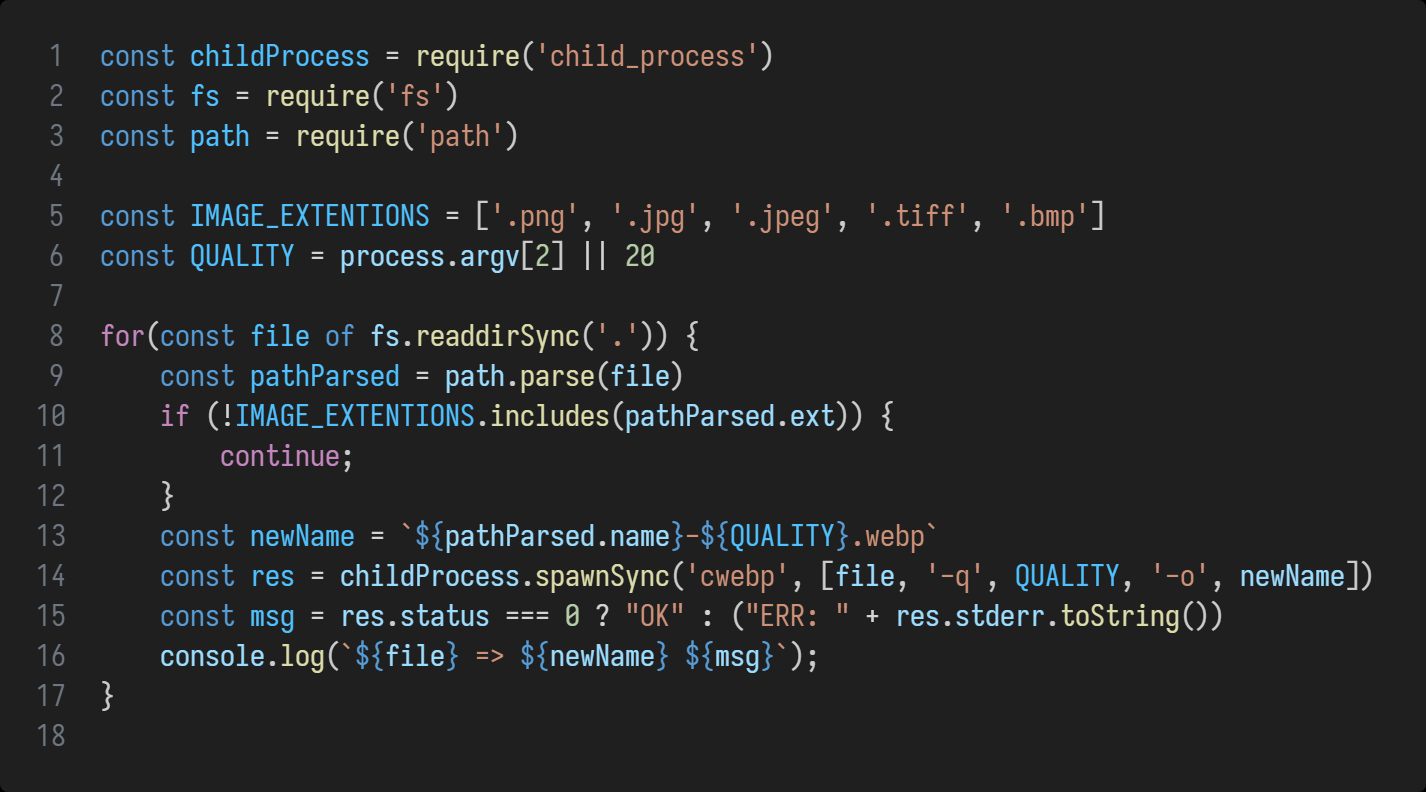
\includegraphics[width=\linewidth]{images/code_script_conv_webm.png}
  \caption{Skrypt konwertujący zdjęcia na format \texttt{WebP}}
  \label{fig:script-webp}
\end{figure}

Po uruchomieniu tego procesu w folderze ze zdjęciami, używając domyślnego parametru jakości równego 20, wygenerowane zostały nowe wersje wszystkich plików zdjęć na stronie. Finalny ich łączny rozmiar to $794.5$KB. W porównaniu do wcześniejszych $46.6$MB, jest to zmniejszenie o $98.3\%$, co jest wielką poprawą.

Można więc przetestować wpływ na wczytywanie witryny, przeprowadzając test \texttt{WebPageTest}'u.

\begin{figure}[H]
  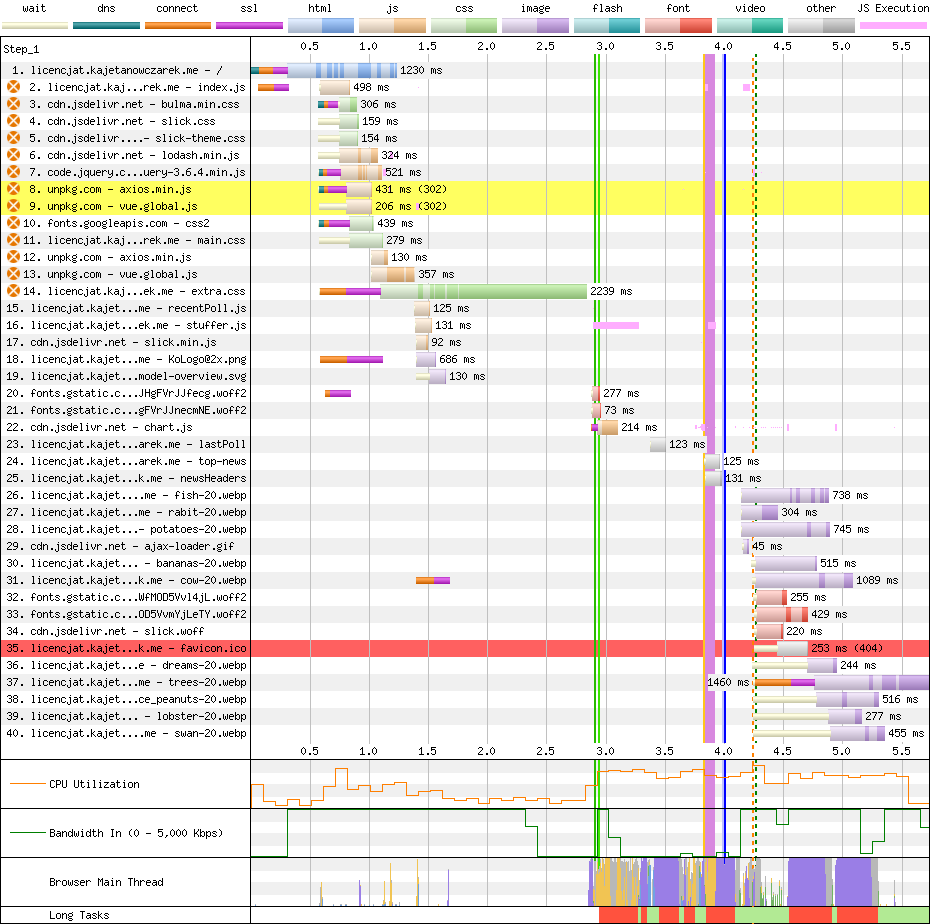
\includegraphics[width=\linewidth]{images/waterfall-after-webp.png}
  \caption{Wyniki testu po zmianie formatu zdjęć z \texttt{PNG} na \texttt{WebP} używając kompresji stratnej}
  \label{fig:waterfall-after-webp}
\end{figure}

Jak widać, zmniejszenie rozmiaru zdjęć o ponad $98\%$ odbiło się na czas wczytywania równie intensywnie, co wartość procentowa by sugerowała. Łączny czas wczytywania strony spadł z ponad $82$s do $5.7$s. Teraz, kiedy wykres nie jest zdominowany przez wczytywanie zdjęć na końcu procesu ładowania witryny, można zauważyć detale tego, co dzieje się w pierwszych sekundach po nawigowaniu na witrynę.

\section{Analiza wczytywania 2}
Dzięki przeskalowaniu wykresu, można ujrzeć dwa elementy, które wcześniej były zbytnio ściśnięte, by móc się im dobrze przyjrzeć. Są nimi wcześniej wspomniane pionowe kreski oraz cienkie elementy wierszy wykresu, repezentujące nawiązywanie połączeń i wykonywanie kodu JavaScript.

Pionowe znaczniki pokazują, kiedy odbywają się kluczowe momenty w procesie wczytywania witryny. 

Chronologicznie pierwsze dwie zielone kreski oznaczają, kiedy przeglądarka rozpocznie proces generowania obrazu do wyświetlenia, oraz kiedy po raz pierwszy rezultaty renderowania strony zostaną pokazane użytkownikowi. 

Następna para, w kolorze pomarańczowym oraz fioletowym, przedstawia wydarzenia zakończenia wczytywania. Pomarańczowa kreska oznacza punkt zmiany stanu gotowości dokumentu na \texttt{interactive}, co oznacza, że wszystkie dane głównego dokumentu HTML zostały już wczytane i przetworzone, ale podzasoby, jak pliki zdjęć, skryptów, stylów czy osadzone dokumenty, mogą jeszcze się wczytywać\footnote{\url{https://html.spec.whatwg.org/multipage/dom.html\#current-document-readiness}}. Od tego momentu, strona jest w stanie reagować na wejścia użytkownika, jak używanie elementów formularzy, ale nie znaczy to, że całość interaktywnej funkcjonalności strony jest już gotowa, jedynie że możliwość użycia takich funkcji przez użytkownika może istnieć dla niektórych witryn. Fioletowy znacznik pokazuje, kiedy było obsługiwane zdarzenie \texttt{DOMContentLoaded}, które jest uruchamiane w reakcji na zmianę stanu gotowości dokumentu. Te dwa wydarzenia powinny zawsze następować bezpośrednio po sobie, natomiast ich szerokość na wykresie oznacza, ile czasu zajęło przetwarzanie tych zmian przez nasłuchujący na nie kod.

Następna para znaczników (acz jeden z nich, jasnoniebieski, nie jest na wykresie dla tej strony pokazany\footnote{Ponieważ strona ta nie używa wydarzenia \texttt{load}, \texttt{WebPageTest} pomija jego znacznik na wykresie. Dla strony która go używa, pojawiłby się on natychmiastowo po ciemnoniebieskiej kresce.}) jest analogiczna do tych właśnie omówionych, ale stan gotowości dokumentu zmienia się na \texttt{complete}, a odpalone wydarzenie to \texttt{load}. Oznaczają one, że główny dokument jak i jego podzasoby został w pełni wczytane i przetworzone. 

Kolejne dwa wskaźniki, tym razem przerywane, pokazują zmiany w wyglądzie dokumentu. Pomarańczowy pokazuje moment znacznych zmian układu strony, kiedy to wiele elementów musiało zmienić swój układ i pozycję. Zielony za to, kiedy nastąpiła największa zmiana w obrazie wyświetlanym przez przeglądarkę\footnote{Choć może się wydawać, że te dwa wydarzenia powinny być tym samym, nie koniecznie musi tak być. Przykładowo, strona może najpierw wczytać skórkę, jak tryb ciemny czy wysokiego kontrastu, powodując zmianę wartości pikseli na całym ekranie, a dopiero później wczytać samą treść, sprawiając, że przeglądarka musi ponownie obliczyć układ dokumentu.}. % usunąłem sekcję o LCP, ale ona still jest zawarta w danych

\begin{figure}[H]
  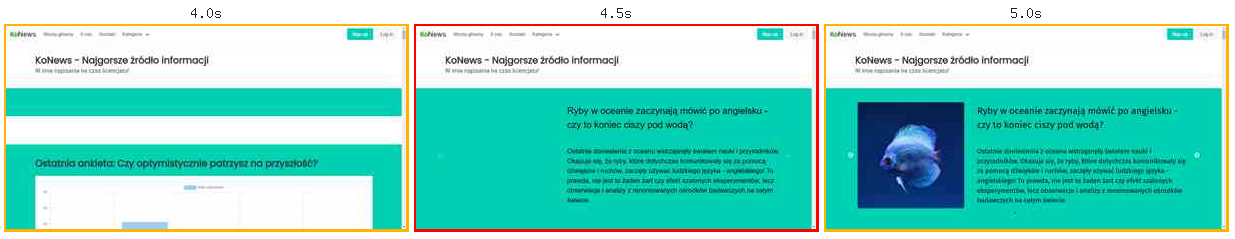
\includegraphics[width=\linewidth]{images/filmstrip.png}
  \caption{Zrzuty ekranu z wczytywania witryny, generowane przez \texttt{WebPageTest}. Wczytanie się zawartości tekstowej po $4.$ sekundzie zmieniło rozmiar nagłówka, przez co zawartość poniżej przesunęła się na stronie, co jest zaznaczone przez pomarańczową przerywaną linię. Wczytanie zawartości zdjęcia do sekundy $5.$ zmieniło wygląd strony, ale nie jej układ.}
  \label{fig:loading-layout-and-lcp}
\end{figure}

\selfnote{Napisać o tym, że LCP daje okazję wymiany całości dokumentu kontra pierwszy widok dokumentu, i czemu może być ok oddać tempo całości, ale zyskać pierwszego widoku} 

%Niektóre z tych metryk są skupione na technicznym aspekcie wczytywania strony, które obchodzą przede wszystkim jej kod kod, oraz użytkowe, które są zauważalne przez użytkowników i wpływają na ich komfort używania witryny. Wymiana, która często pojawia się w dziedzinie optymalizacji, to wybór między szybszym wczytaniem całości strony, a przygotowaniem minimum używalnego dla użytkownika. Patrząc na czas do LCP, ponieważ nie cała stona jest wyświetlana na raz, można podjąć decyzję, aby poświęcić treści niżej na stronie, wczytująć je z mniejszym priorytetem, ale skracając czekanie na pokazanie się wstępnego wycinka zawartości, aby użytkownik mógł już mieć cokolwiek używalnego, w trakcie gdy reszta witryny dalej się wczytuje.

%Na przykładowym projekcie, na którym prezentuję te techniki, zostały jeszcze okazje, by przyśpieszyć wczytywanie strony w spósób całkowity, ale po zastosowaniu tych zmian, skupię się miejscami na przyśpieszeniu wczytywania z perspektywy użytkownika, czyli kiedy strona wyświetla się i jest używalna, nawet jeżeli nie ma jeszcze pełni treści. Miejscami może to pogorszyć to czas do wczytania całości strony, ale poprawi subiektywne odczucie szybkości witryny, które starają się zmierzyć niektóre omówione heurystyki.

\section{Zmienianie rozmiarów zdjęć}

Oprócz kompresji zdjęć, można zastosować jeszcze jedną taktykę na zmniejszenie ich kontrybucji w przesyle danych. Jest tym wybranie bardziej adekwatnych rozmiarów. Aktualna wersja witryny używa zdjęć w rozmiarze $2048\times2048$ pikseli, natomiast na wielu ekranach zdjęcia nie są nawet połowy tego rozmiaru.

Do zmiany rozmiaru zdjęć można użyć tego samego narzędzia, które zostało użyte do skompresowania zdjęć do formatu WebP, gdyż posiada ono też opcje wycinania i zmiany rozmiaru zdjęć. Zmodyfikowano więc skrypt do konwersji, aby generował też obrazy o różnych, zadanych rozmiarach. 
Dzięki tej zmianie, skrypt generuje warianty tego samego zdjęcia, ale z innymi nazwami i rozmiarami.

\begin{figure}[H]
  \centering
  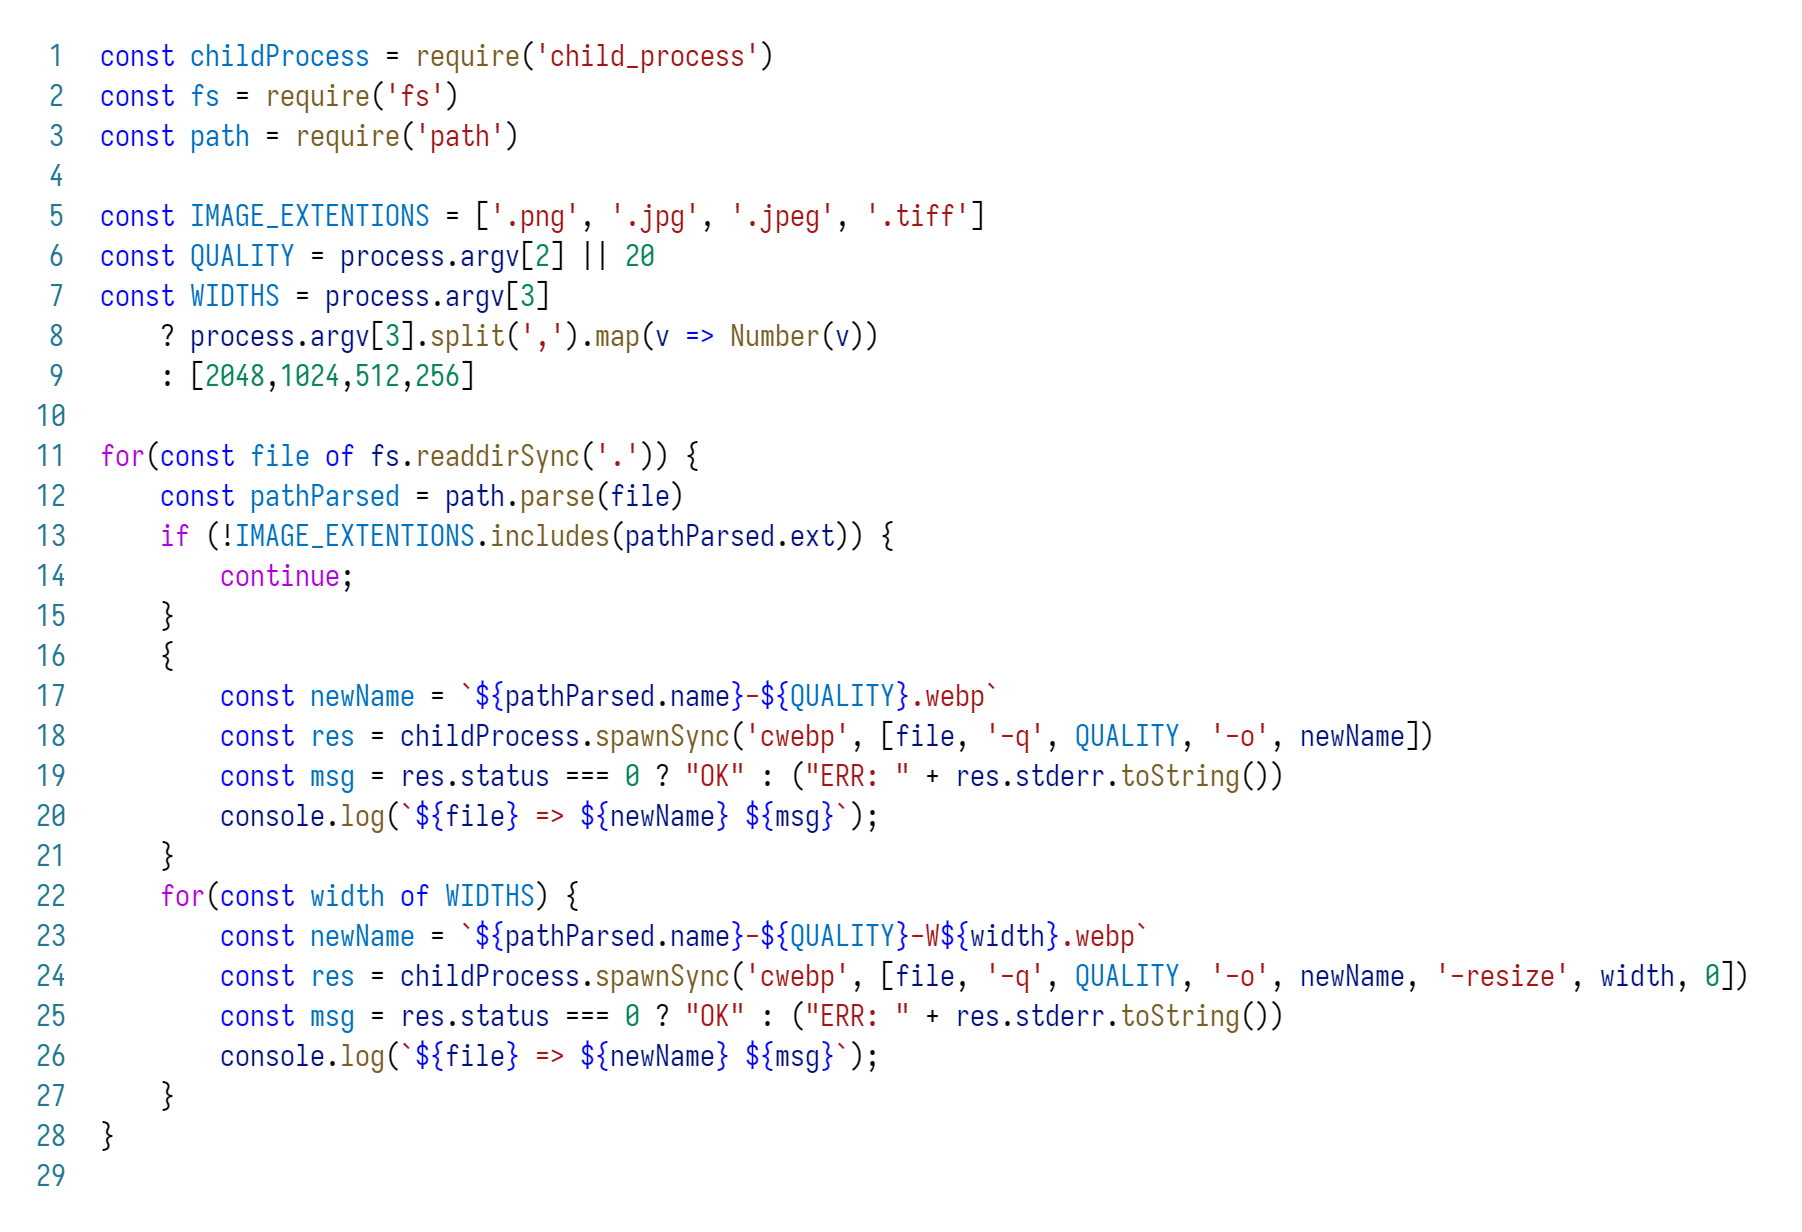
\includegraphics[width=\linewidth]{images/code_script_conv_format_and_size.png}
  \caption{Skrypt konwertujący format pliku, oraz generujący warianty w różnych rozmiarach}
  \label{fig:script-format-and-size}
\end{figure}

Mając takie pliki, można sprawić, że przeglądarka będzie wybierała optymalne rozmiarowo pliki dla danego urządzenia. Można to osiągnąć, modyfikując elementy \texttt{<img>}, aby używały atrybutów \texttt{srcset}\footnote{\url{https://html.spec.whatwg.org/multipage/images.html\#srcset-attribute}} oraz \texttt{sizes}, lub zamienić te elementy na elementy \texttt{picture}\footnote{\url{https://html.spec.whatwg.org/multipage/embedded-content.html\#the-picture-element}} oraz \texttt{source}. Tutaj zaprezentowana zostanie druga metoda, ale obie polegają na wyrażeniu tego samego mechanizmu za pomocą różnej składni.

W połączeniu, elementy \texttt{picture} oraz \texttt{source} pozwalają wyświetlać w ramach jednego elementu na stronie różne pliki zdjęć, wybrane na bazie \texttt{CSS}'owych kwerend \texttt{media}\footnote{\url{https://www.w3.org/TR/mediaqueries-4/}}. Można więc w ramach jednego elementu \texttt{picture} dostarczać wiele różnych źródeł oraz warunki, które muszą być spełnione, aby dane źródło było użyte. Można więc przeanalizować, dla jakich układów strony potrzebne są jakie rozdzielczości zdjęć, i stworzyć zestaw formatów, które sprawią, że do klienta będzie przesyłane nie więcej danych obrazów niż potrzeba.

Dla przykładowego projektu wybór optymalnej rozdzielczości nie jest prosty. Jak widać na rys. \ref{fig:frontpage-articles}, na szerokim, komputerowym monitorze, część zdjęć jest wyświetlana w układzie z trzema kolumnami. Natomiast na ekranie o wiele węższym, na przykład komórkowym, kolumny znikają, a karta artykułu, w tym zdjęcie, zajmuje całą szerokość ekranu. Przez to zachowanie, w miarę zmniejszania się ekranu wymagana rozdzielczość zdjęć maleje, ale w pewnym momencie (kiedy wyłącza się układ kolumnowy) rośnie.

\begin{figure}[H]
  \centering
  
\includegraphics[width=\linewidth/\real{3.5}]{images/screenshot-iphone11.png}
  \caption{Układ witryny dla ekranów mobilnych (rozmiar ekranu iPhone 11)}
  \label{fig:screenshot-iphone11}
\end{figure}

Dodatkowo że na bardzo szerokich monitorach zawartość strony jest centrowana, zostawiając przestrzeń po bokach. Oznacza to, że od pewnej szerokości ekranu w górę, zdjęcia będą takiego samego rozmiaru. 

\begin{figure}[H]
  
\includegraphics[width=\linewidth]{images/screenshot-very-wide.png}
  \caption{Układ witryny dla bardzo szerokich ekranów}
  \label{fig:screenshot-verywide}
\end{figure}

Wiedząc, przy użyciu jakiej technologii zbudowana została ta strona (framework \texttt{CSS} o nazwie \texttt{Bulma}), oraz że nie były modyfikowane jej ustawienia, można ustalić, że tą maksymalną szerokością ekranu jest $1408$ pikseli\footnote{\href{https://web.archive.org/web/20230518134357/https://bulma.io/documentation/layout/}{\texttt{https://bulma.io/documentation/layout/}}}, przy którym centrowana treść dostaje szerokość $1344$ pikseli. W podobny sposób można sprawdzić, że układ kolumnowy wyłącza się na ekranach mniejszych niż $768$ pikseli\footnote{\href{https://web.archive.org/web/20230512141342/https://bulma.io/documentation/overview/responsiveness/}{\texttt{https://bulma.io/documentation/overview/responsiveness/}}}.

Wiedząc, jaki jest kod witryny, możemy policzyć, ile dokładnie miejsca zajmie dane zdjęcie przy konkretnej szerokości ekranu. Można też użyć skryptów lub narzędzi developera, aby zmierzyć szerokości elementu wyświetlanego przez przeglądarkę.

\begin{figure}[H]
  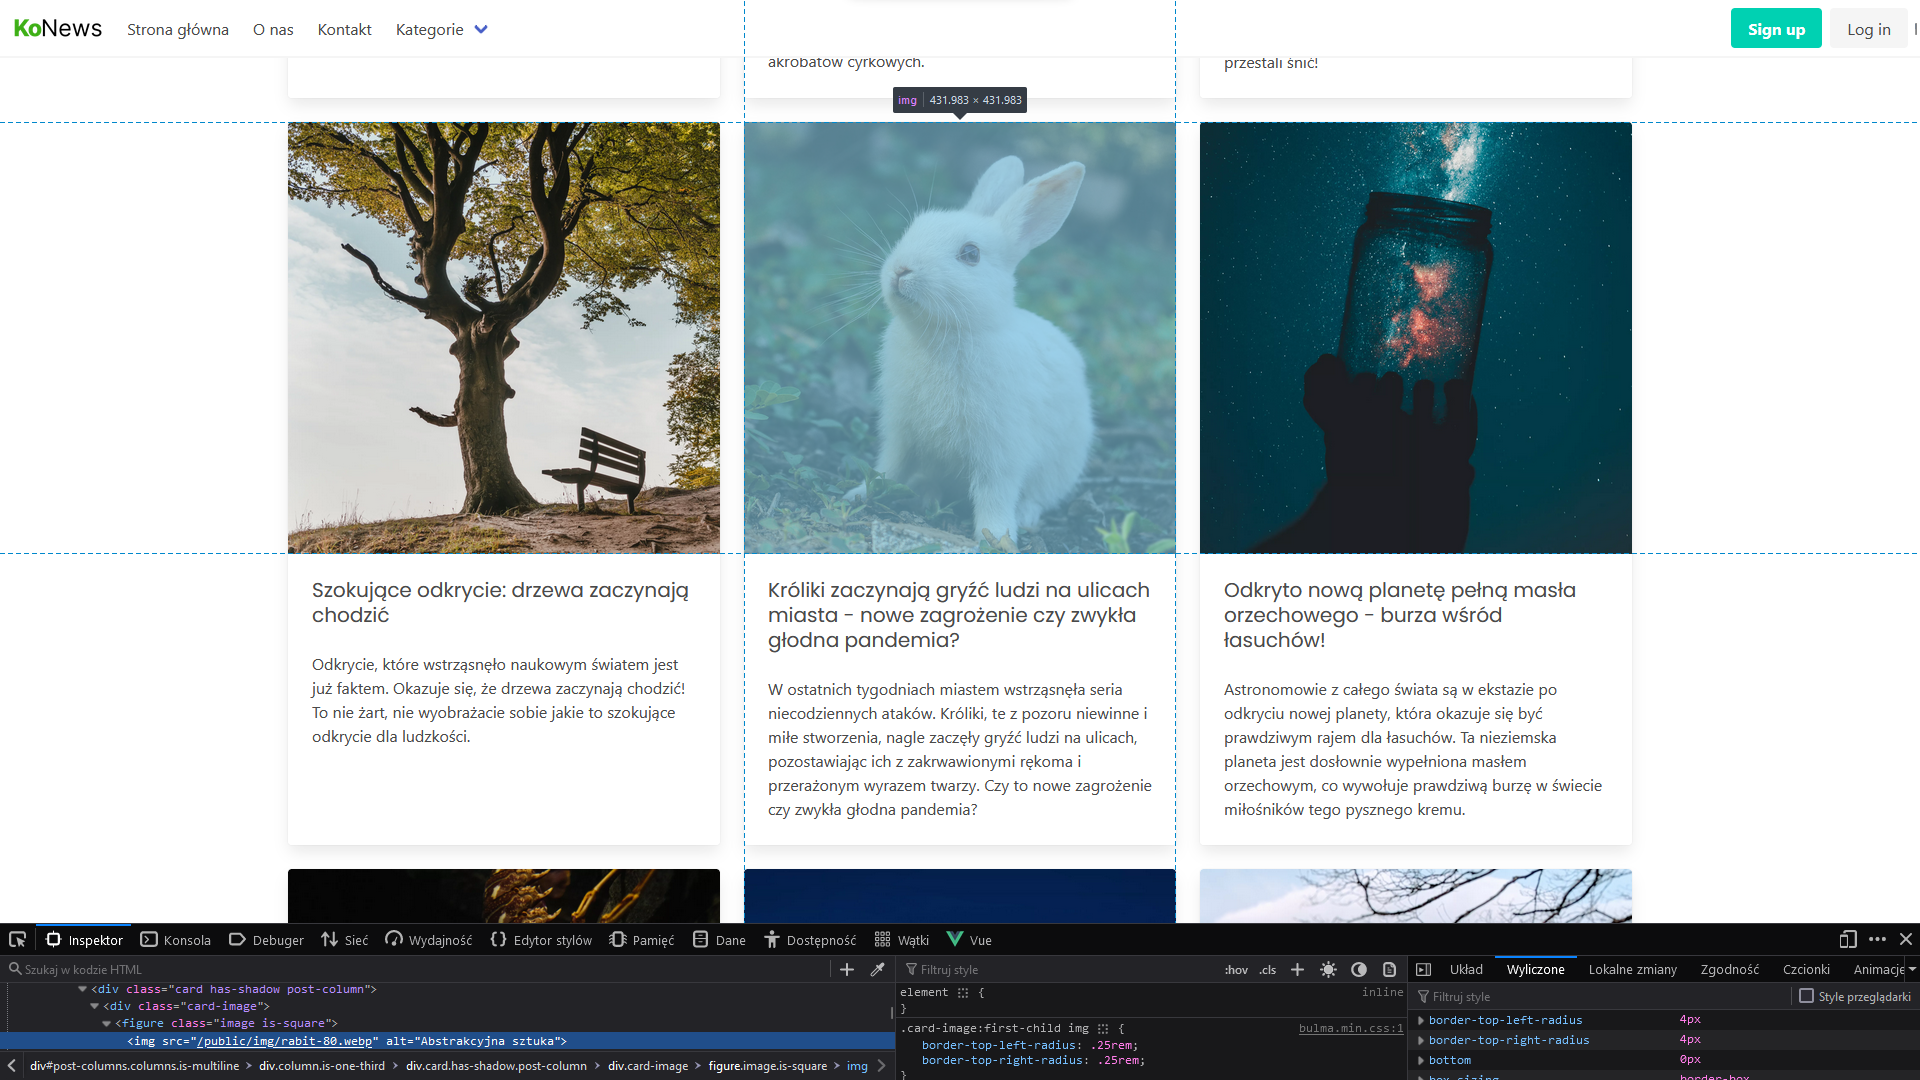
\includegraphics[width=\linewidth]{images/screenshot-devtools-1080width.png}
  \caption{Mierzenie rozmiaru zdjęcia za pomocą narzędzi developera. Tutaj, dla ekranu $1920\times1080$, zdjęcie jest kwadratem o boku ledwo co poniżej $432$ pikseli.}
  \label{fig:screenshot-measuring}
\end{figure}

Mierząc rozmiary tych elementów dla różnych rozmiarów ekranu, otrzymano następujące wyniki:

\begin{center}
  \begin{tabular}{|c|c|}
    \hline
    Szerokość ekranu (w pikselach) & Rozmiar zdjęcia (w pikselach) \\
    \hline
    $2560$ (Quad HD) & $432$ \\
    $1920$ (Full HD) & $432$ \\
    $1366$ & $368$ \\
    $1280$ (HD) & $368$ \\
    $1023$ (największy rozmiar tabletowy) & $309$ \\
    $770$ (najmniejszy niemobilny) & $225$ \\
    $769$ (mobilne wg Bulmy) & $720$ \\
    $640$ (SD) & $592$ \\
    $500$ & $452$ \\
    $320$ (iPhone 3) & $272$ \\
    $300$ & $252$ \\
    $200$ & $252$ \\
    \hline
  \end{tabular}
\end{center}

Jak widać, przez wyłączenie się systemu kolumn na ekranach mobilnych, zdjęcia na węższych ekranach są większe, niż na dowolnie dużych. Dla dużych desktopowych rozdzielczości, Bulma przeskakuje między rozmiarami $432$ dla Full HD i $368$ dla zwykłego HD pikseli (aczkolwiek jest niewielkie okno rozmiarów ekranu, gdzie pomiędzy tymi dwoma rozdzielczościami zdjęcia mają inne, delikatnie mniejsze od $432$ rozmiary). Najmniejsze zdjęcie, jakie wyświetli się na niemobilnym ekranie ma bok $225$ pikseli, gdyż przy delikatnie mniejszym ekranie rozmiar zdjęcia wzrośnie do największego, jaki kiedykolwiek się wyświetli, czyli $720$ pikseli wysokości i szerokości. W formacie mobilnym zdjęcia maleją w równym tempie co ekran, będąc o $48$ pikseli mniejsze niż jego szerokość, aż do minimum $252$ pikseli.

Można więc wyznaczyć zestaw rozmiarów, które obsłużą potrzebne zakresy rozmiarów ekranu. Można generować niezliczone różne rozdzielczości, ale na potrzeby tej strony wystarczający wydaje się zestaw:

\begin{itemize}
  \item $720$ pikseli, dla dużych telefonów,
  \item $432$ piksele, dla dużych komputerów i średnich telefonów,
  \item $368$ pikseli, dla mniejszych komputerów i małych telefonów.
\end{itemize}
 
Po wygenerowaniu plików zdjęć o zadanych rozmiarach za pomocą skryptu, trzeba też dodać obsługę zmiennych rozmiarów w kodzie witryny. Do generowania elementów artykułów na stronie używany jest framework Vue. Trzeba więc zmienić wzorzec, który jest używany przez kod do dynamicznej generacji treści.

\begin{figure}[H]
  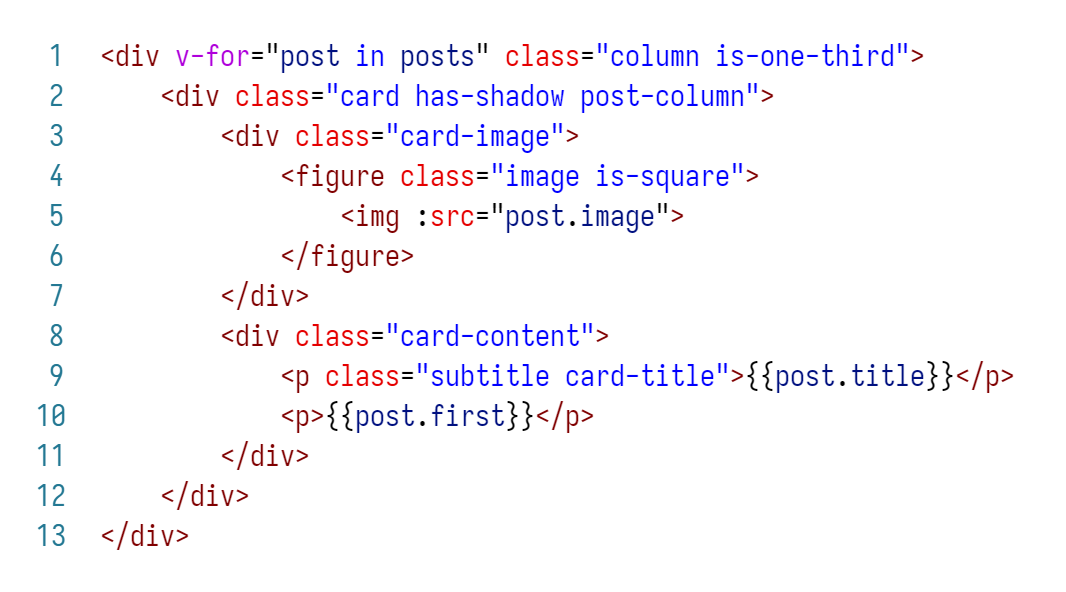
\includegraphics[width=\linewidth]{images/code-vue-image-card-old.png}
  \caption{Wzorzec Vue generujący karty z artykułami}
  \label{fig:code-vue-template-articles-old}
\end{figure}

W środku tego wzorca, znajduje się element \texttt{<img>}, którego właściwość \texttt{src} jest dynamicznie ustawiana przez Vue na konkretną, zadaną wartość (Znak \texttt{:} jest używany w Vue do oznaczania właściwości dynamicznych. Tutaj, jest to pole \texttt{image} na obiekcie \texttt{post}.)

Trzeba stworzyć mechanizm wybierający, które zdjęcie ma być wysłane z serwera. W przypadku tego projektu zdecydowano, żeby serwer wysyłał adres \texttt{URL} zdjęcia z tekstem \texttt{WIDTH} w miejscu, w które należy wstawić żądaną szerokość obrazu. Kod na stronie będzie musiał więc podmieniać ten ciąg na dany rozmiar w pikselach.

W celu implementacji takiego mechanizmu, należy obwinąć element \texttt{<img>} w element \texttt{<picture>}. W takiej konfiguracji, jeżeli mechanizm wybierania lepiej dopasowanych treści nie wybierze żadnego zasobu, to element \texttt{<img>} zostanie użyty jako domyślna wartość.

Wewnątrz elementu \texttt{<picture>} można zamieścić elementy \texttt{<source>}, które opisują alternatywne źródła plików obrazów. W przeciwieństwie do elementów \texttt{<img>}, używają one atrybutu \texttt{srcset} zamiast \texttt{src}.

Można więc stworzyć następujący wzorzec:

\begin{figure}[H]
  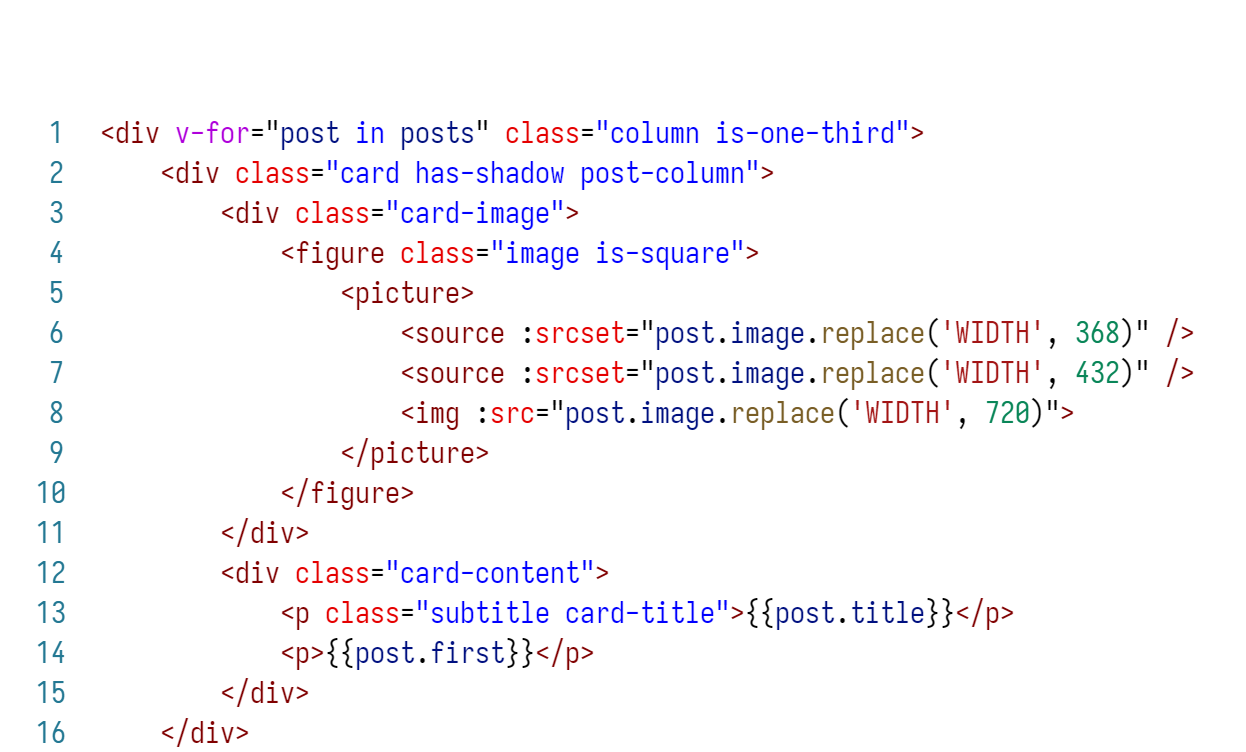
\includegraphics[width=\linewidth]{images/code-vue-image-card-mid.png}
  \caption{Wzorzec częściowo zmodyfikowany, aby używać responsywnych obrazów}
  \label{fig:code-vue-template-articles-mid}
\end{figure}

Nie jest to jeszcze pełne rozwiązanie. Gdyby otworzyć teraz witrynę, wyświetliło by się wiele rozmytych zdjęć. Wynika to z tego, że nie podano kwerend \texttt{media}, które ustalałyby, które ze źródeł wybrać do wyświetlenia. Trzeba więc wybrać, w jakim zakresie szerokości ekranów mają być użyte dane obrazy. Patrząc na poprzednie analizy, można stwierdzić, że:

\begin{itemize}
  \item Zdjęcia o szerokości $368$ pikseli powinny być użyte na ekranach szerszych niż $769$, ale węższych lub równych $1366$ pikseli, oraz na węższych niż $416$ pikseli,
  \item Zdjęcia o szerokości $432$ pikseli powinny być użyte na ekranach o szerokości ponad $1366$ pikseli, oraz na szerszych niż $416$, ale węższych niż $480$ pikseli
  \item Zdjęcia o szerokości $720$ pikseli powinny być używane na ekranach węższych lub równych $769$, ale szerszych niż $480$ pikseli
\end{itemize}

Źródłą i ich warunki są testowane od pierwszego w kodzie do ostatniego, zatrzymując się na pierwszym, na który kwerenda \texttt{media} zezwala.
Ponieważ według wcześniejszych wyborów dotyczących warunków selekcji danych rozmiarów, warunki wyświetlenia rozmiaru $720\text{px}$ są rozłączne do pozostałych dwóch, może on zostać domyślnym źródłem, będąc ustawionym przez element \texttt{<img>}.  

%\selfnote{Napisać o tym, że ten mechanizm działa na bazie szerokości}

Rozmiar $368\text{px}$ jest preferowany dla szerokości z zakresu $\rinterval{0}{416\text{px}} \cup \linterval{769\text{px}}{1366\text{px}}$. Żeby przekonwertować zakres zamknięty $\interval{a}{b}$ na kwerendę \texttt{media}, odpowiadający kod to \texttt{(min-width: a) and (max-width: b)}. Niestety nie ma sposobu, żeby przekonwertować zakres otwarty, trzeba więc użyć zakresu zamkniętego z jedną z granic przesuniętą o jeden piksel. Jeżeli dolna granica to zero, oraz kiedy górna jest w nieskończoności, możemy pominąć ich część kodu\footnote{Tworząc więc kwerendy jak \texttt{(min-width: a)} lub jak \texttt{(max-width: b)}}. Aby zapisać, że dane źródło jest preferowane dla więcej niż jednej kwerendy, tutaj reprezentujących zakresy szerokości, można postawić kody tych kwerend po przecinku.

Wedle powyższego, kwerenda \texttt{media}, która wyświetli zdjęcie o szerokości $368\text{px}$, zgodnie z wyżej opisanymi wymaganiami, to:
\begin{verbatim}
  (max-width: 416px), (min-width: 770px) and (max-width: 1366px)
\end{verbatim}
Podobnie możemy napisać kwerendę dla zdjęć o szerokości $432\text{px}$:
\begin{verbatim}
  (min-width: 417px) and (max-width: 480px), (min-width: 1367px)
\end{verbatim}
Dla pozostałych przypadków wybierane jest domyślne źródło. 

Są to już wszystkie elementy, żeby w pełni zaimplementować responsywne dopasowywanie rozmiaru zdjęć. Łącząc je w jedność, otrzymano następujący kod:

\begin{figure}[H]
  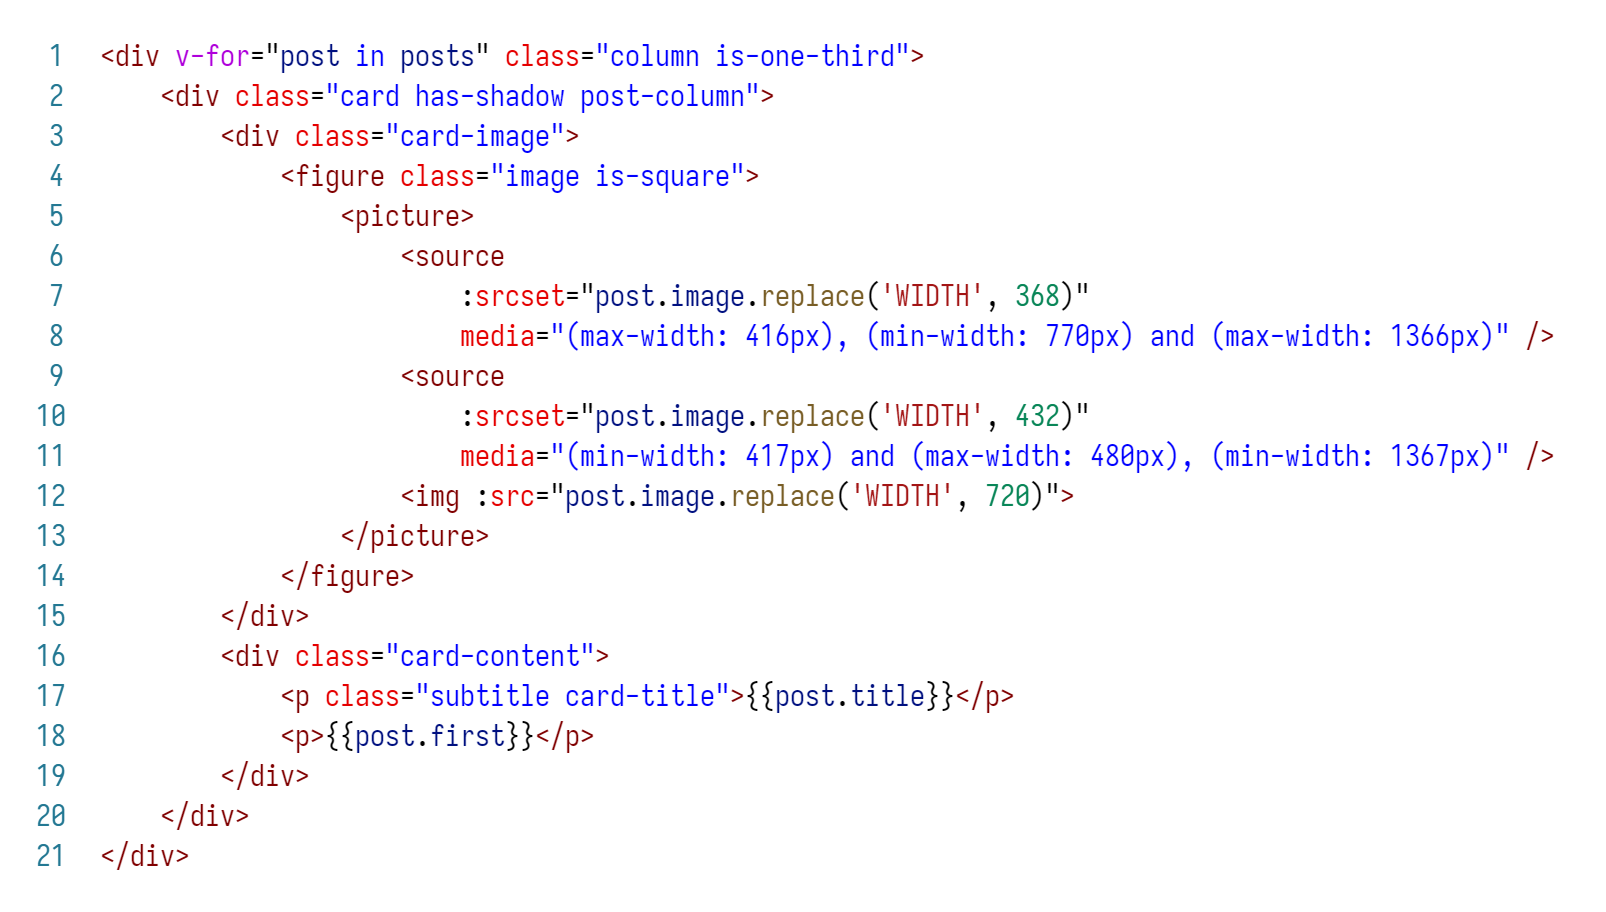
\includegraphics[width=\linewidth]{images/code-vue-image-card-done.png}
  \caption{Zakończony wzorzec, który wybiera zdjęcia o optymalnie małym rozmiarze, aby przesłać jak najmniej danych}
  \label{fig:code-vue-template-articles-done}
\end{figure}

Niefortunnym aspektem tej optymalizacji jest to, że testy witryn korzystających z niej przynoszą nieco inne efekty dla różnych konfiguracji tego samego sprzętu. Mechanizm korzysta z szerokości ekranu aby ustalić, jakie źródło dla obrazu wybrać, tak jest to prawdą tylko kiedy okno przeglądarki zajmuje całą szerokość ekranu. Jeżeli zajmuje ono tylko jakąś część ekranu, na przykład przez wyświetlenie w okienku, to tylko ta część jest traktowana w ramach mechanizmu wyboru.

Testując te zmiany przy użyciu WebPageTest'u, otrzymano następujące wyniki:

\begin{figure}[H]
  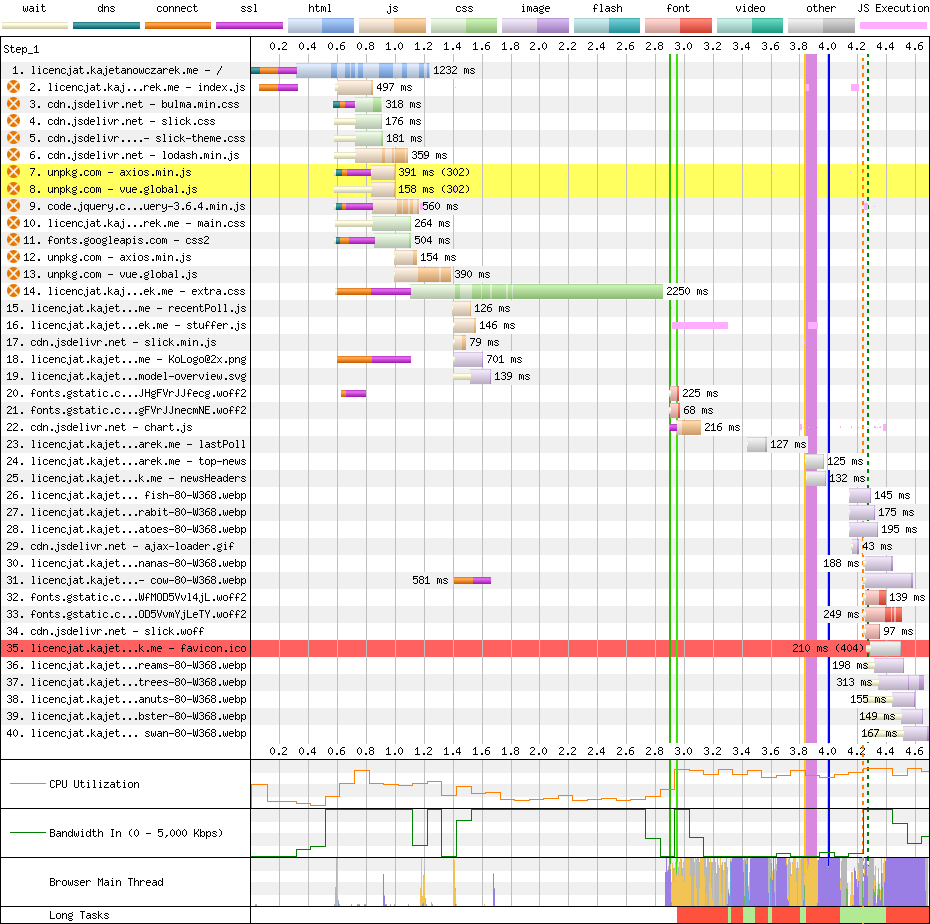
\includegraphics[width=\linewidth]{images/waterfall-after-sizing.png}
  \caption{Wyniki testów po wdrożeniu responsywnego wyboru zdjęć}
  \label{fig:waterfall-after-sizing}
\end{figure}

Porównując z poprzednim testem, łączny czas wczytywania strony spadł z $5.7\text{sek}$ do $4.7\text{sek}$, więc udało się odzyskać sekundę czasu przy każdym wczytaniu strony. Ponieważ zdjęcia nie blokowały pierwszego wyświetlenia, ani nie powodowały oczekiwania na ich wczytanie, aby móc korzystać z interaktywności, zmiany te nie poprawiły pozostałych metryk. Niezmiennie, jest to poprawa czasu, jak i oszczędności kosztu transferu danych, a choć czas do zobaczenia przez użytkownika jakieś treści na witrynie nie jest mniejszy, tak mniej czasu będzie spędzone na patrzeniu się na niewczytane lub częściowo wczytane zdjęcia, więc poprawiono używalność podczas wczytywania witryny.

Alternatywnym sposobem, aby zrealizować podobny efekt optymalizacji, byłoby najpierw wczytywanie zasobów w niskiej rozdzielczości, a kiedy strona będzie już w pełni wczytana, zacząć zamieniać ja wersje o wyższej rozdzielczości. Nie zostanie tutaj omówione, jak zastosować tą technikę, gdyż ma ona ograniczone wsparcie wśród standardów webowych, więc całość implementacji jest po stronie twórcy witryny.


\section{Użycie kompresji bezstratnej}

Póki co użyto kompresji zdjęć, aby znacznie zmniejszyć rozmiar plików witryny. Była to kompresja stratna, gdyż nie wszystkie detale oryginalnych zdjęć zachowały się przez cały proces, lecz dalej zawarte jest ich wystarczająco dużo, aby obrazy były czytelne. Takiego rodzaju kompresji nie możemy zastosować do kodu strony, gdyż każdy ich detal jest kluczowy dla poprawnego funkcjonowania witryny. Możemy jednak użyć kompresji bezstratnej.

Istnieje wiele różnych algorytmów na bezstratną kompresję danych, ale w ramach tego projektu użyto formatu plików \texttt{gzip}, który wykorzystuje algorytm kompresji \texttt{DEFLATE}\footnote{\url{https://www.ietf.org/rfc/rfc1952.txt}, strona 5}.

Algorytm \texttt{DEFLATE} kompresuje dane w dwóch krokach. Pierwszy, to bazowany na algorytmie \texttt{Lempel-Ziv77} mechanizm usuwania powtórzeń, który zastępuje nie pierwsze wystąpienia sekwencji bajtów odniesieniami do ich poprzednich wystąpień. Drugi, to rozszerzenie kodowania Huffmana, które poświęca prostotę przetwarzania w modelu "1 bajt, kodujący jeden znak\footnote{Kodowania, gdzie 1 bajt to jeden znak są popularne, acz definitywnie nie są jedynym systemem. \texttt{ASCII} koduje jeden znak w $7$miu bitach, natomiast \texttt{Unicode} korzysta ze zmiennej ilości bajtów do przedstawienia jednego symbolu.}, w równych odstępach" na rzecz systemu korzystającego ze zmiennej długości bitowej znaku, nadając najpowszechniej występującym znakom krótsze reprezentacje. Rozszerzenie użyte w algorytmie \texttt{DEFLATE} polega na dodaniu do drzewa Huffmana znaków nie reprezentujących danych, a rodzaje odniesień wygenerowanych przez pierwszy krok.

Ponieważ algorytmy te są powszechnie używane w Internecie, obsługa ich w bardzo wielu przypadkach powinna być bardzo prosta. Serwer, który obsługuje testową witrynę, korzysta z programu \texttt{nginx}. Żeby włączyć obsługę kompersji \texttt{gzip}, wystarczy zmodyfikować plik konfiguracji tego serwera, dodając dyrektywy \texttt{gzip on;} oraz ustawiając rodzaje odpowiedzi, które powinny być kompresowane. Taki plik konfiguracji może wyglądać następująco:
\begin{figure}[H]
  \centering
  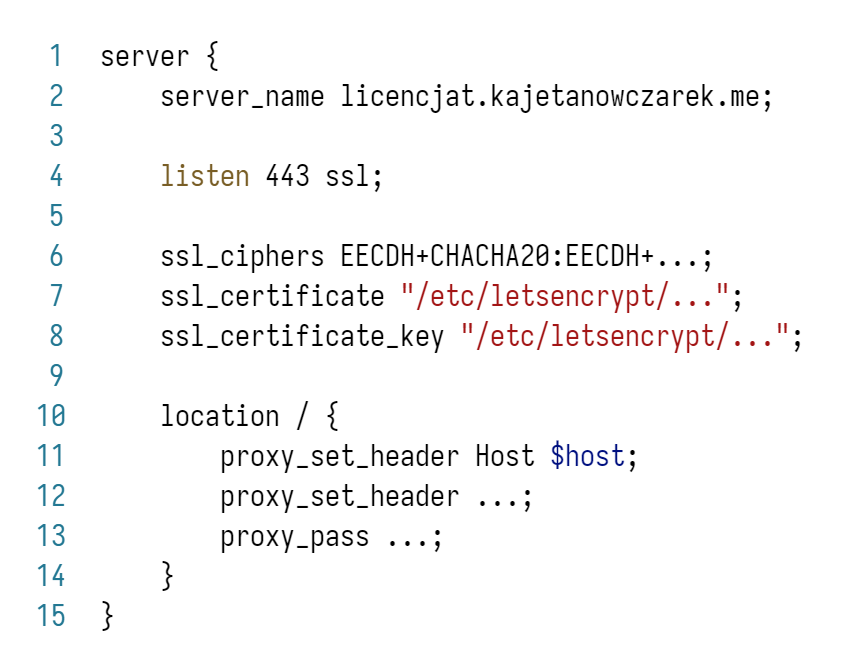
\includegraphics[width=\linewidth/\real{1.55}]{images/code-nginx-conf-trunc-nogzip.png}
  \caption{Plik konfiguracji nginx, używany przez prawdziwy serwer, z którego pochodzą wyniki pomiarów, z pominiętymi danymi zbędnymi do tego tematu.}
  \label{fig:nginx-before-gzip}
\end{figure}
Można dodać obsługę kompresowania do formatu \texttt{gzip} plików \texttt{HTML}, \texttt{CSS} i \texttt{JavaScript}, zmieniając zawartość tego pliku na:
\begin{figure}[H]
  \centering
  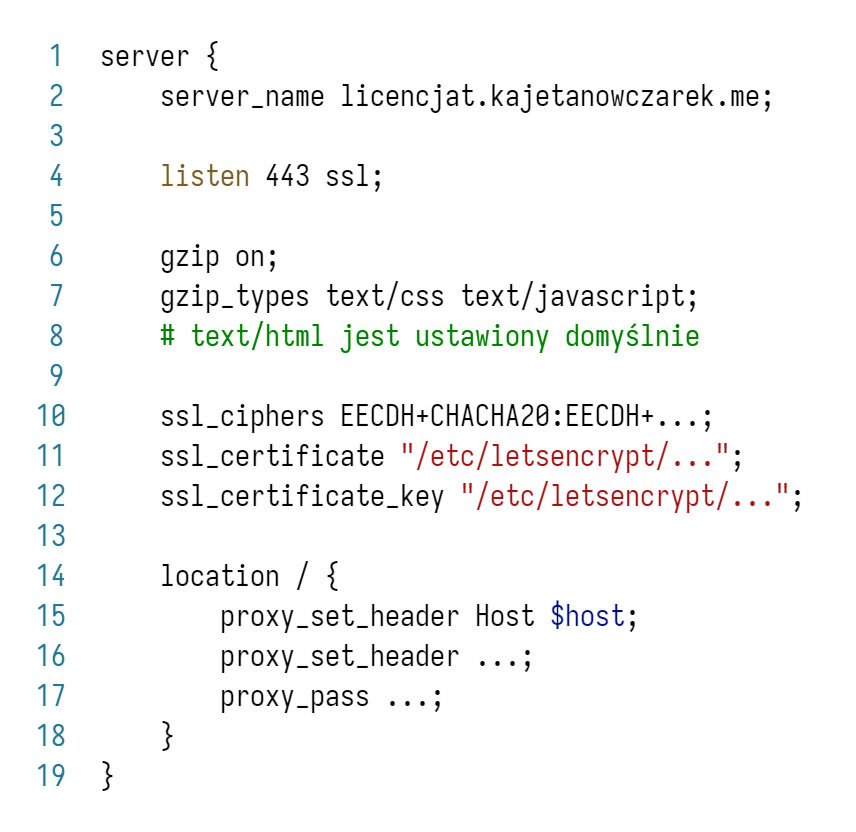
\includegraphics[width=\linewidth/\real{1.55}]{images/code-nginx-conf-trunc-gzip.png}
  \caption{Zmodyfikowany plik konfiguracji nginx, uruchamiający kompresję \texttt{gzip} odpowiedzi o formacie \texttt{MIME} \texttt{text/html}, \texttt{text/css} i \texttt{text/javascript}.}
  \label{fig:nginx-after-gzip}
\end{figure}

Po zastosowaniu takich zmian otrzymano następujące wyniki:
\begin{figure}[H]
  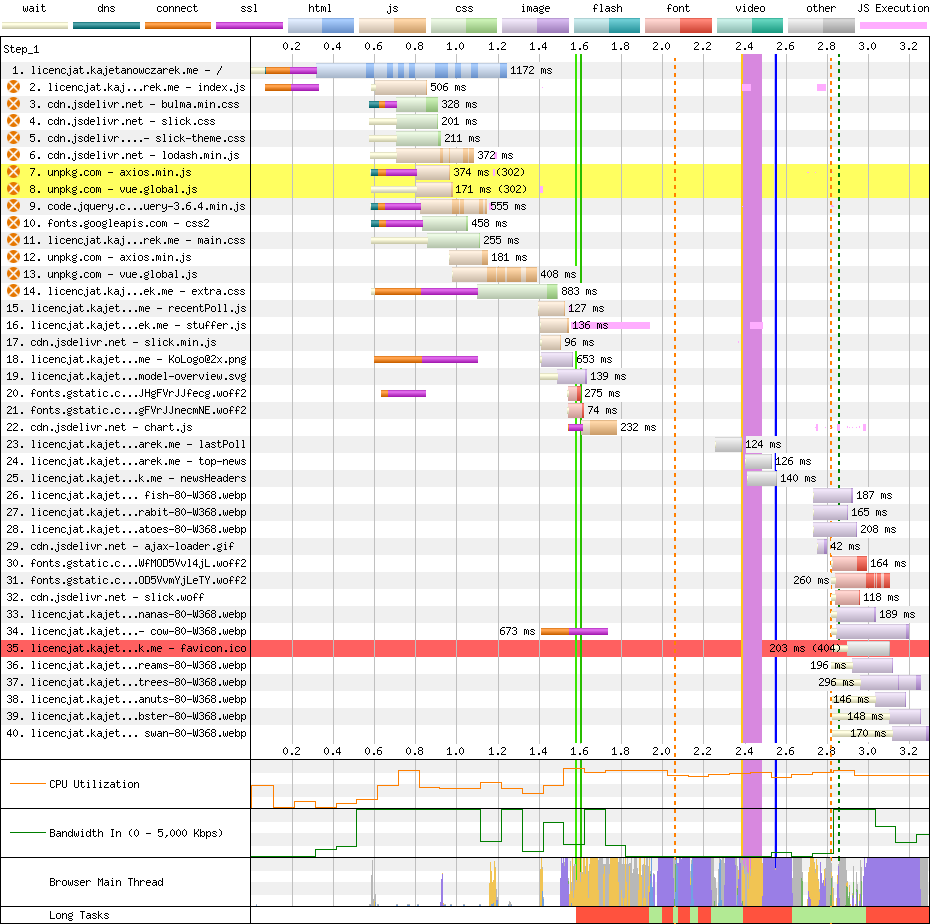
\includegraphics[width=\linewidth]{images/waterfall-after-gzip.png}
  \caption{Wyniki testów WebPageTest po uruchomieniu kompresji \texttt{gzip}}
  \label{fig:waterfall-after-gzip}
\end{figure}

Jak można zauważyć, największym źródłem poprawy czasu wczytywania jest znaczne przyśpieszenie wczytywania pliku \texttt{extra.css}. Prócz tego, poprawy są bardzo ograniczone, co wynika z tego, że duża część zasobów tego typu nie była wysyłana przez modyfikowany właśnie serwer, a przez serwery usług \texttt{jsdelivr} oraz \texttt{unpkg}, które dostarczają pliki wielu bibliotek, w tym te używane przez witrynę testową. Ponieważ połączenie jest nawiązywane z innym serwerem, włączenie kompresji na tym nie wpływa na to, jak zostaną wykonane te połączenia.




\section{Sprytniejsze stylowanie}

Kontynuując poprawianie witryny, można zwrócić uwagę do zasobów \texttt{CSS}. Choć po skompresowaniu, plik \texttt{extra.css} nie zabiera tak wiele czasu jak wcześniej, tak jest on drugim najdłużej wczytywanym plikiem, zaraz po głównym dokumencie. Ponieważ pliki \texttt{CSS}, które opisują, jak elementy witryny mają wyglądać na ekranie, blokują wyświetlanie użytkownikowi zawartości strony\footnote{\url{https://html.spec.whatwg.org/\#render-blocking-mechanism}}, przyśpieszenie czasu ich wczytania sprawi, że na witrynie treści zostaną przedstawione użytkownikowi wcześniej.

Przyglądając się waterfallowi z rysunku \ref{fig:waterfall-after-gzip}, można zauważyć, że większość zielonych prostokątów, oznaczających zapytania pobierające pliki \texttt{CSS}, jest w swojej bladej wariacji kolorowej. Oznacza to, że niewiele czasu zostało poświęcone na pobieranie, a wiele na czekanie na dane. Dodatkowo, cieńsze białe kreski przed zielonymi prostokątami pokazują, że zapytania te nie były w stanie przejść natychmiastowo do gotowości do pobierania, a musiały poczekać na skończenie innych aktywności. 

Pomimo tego, że większość czasu poświęconego na arkusze stylów był spędzony na czekaniu, możemy zauważyć dwa bloki bardziej nasyconego zielonego. Pierwszy jest częścią pobierania pliku \texttt{bulma.min.css}, który zawiera używaną przez projekt bibliotekę, zbitą w jeden plik zawierający jej całość. Drugi za to jest powiązany z plikiem \texttt{extra.css}, który jest częścią nie bibliotecznego kodu projektu.

Plik \texttt{extra.css} przedstawia bibliotekę CSS'ową, która zawiera wiele tzw. \emph{utility classes}, czyli klas obiektów pozwalających na dostosowanie wyglądu elementów wyłącznie z poziomu kodu HTML, poprzez użycie wielu klas zawierających w swojej nazwie żądany parametr. W przypadku tego projektu, używane są dwa rodzaje takich klas\footnote{Choć te dwa przypadki są definitywnie przesadzone w skali ilości opcji parametrów, mają one przestawiać odpowiednik wielu mniejszych klas. Ignorując nieco detali związanych z kompresją, można zająć podobną ilość danych, używając wielu utility class o mniejszej liczbie opcji na ich parametry.} - trójka klas \texttt{luma-\#}, \texttt{luma-bg-\#} oraz \texttt{fix-text}, oraz element siatki, otrzymujący dwa parametry w dwóch klasach, \texttt{row-\#} oraz \texttt{col-\#}.

Klasa \texttt{luma-\#}, gdzie \texttt{\#} to liczba od $0$ do $255$, po dodaniu do elementu sprawia, że zawarty tekst przyjmuje kolor w odcieni szarości zależny od liczby \texttt{\#}, poprzez nadanie mu koloru z przestrzeni \texttt{RGB}, z wartościami wszystkich kanałów ustawionymi na \texttt{\#}. Klasa \texttt{luma-bg-\#} wybiera ten sam kolor, co \texttt{luma-\#}, jednak ustawia go na kolor tła, a nie tekstu. Klasa \texttt{fix-text}, kiedy jest ustawiona na elemencie z \texttt{luma-bg-\#}, lub kiedy element dziedziczny takowego ją posiada, ustawia tekst na kontrastujący - biały dla $\texttt{\#} < 127$, czarny dla $\texttt{\#} \geq 127$.

\begin{figure}[H]
  \centering
  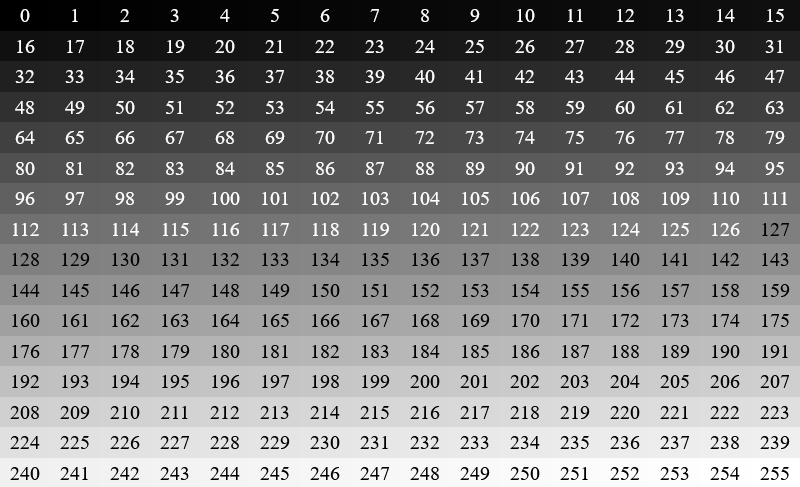
\includegraphics[width=\linewidth]{images/ui-luma-grid.png}
  \caption{Żądany efekt - elementy zawierające tekst z wartością użytego parametru, na które nałożono klasy \texttt{luma-\#} oraz \texttt{fix-text}}
  \label{fig:ui-luma-grid}
\end{figure}

Sposoby na osiągnięcie takiej funkcjonalności dla wielu przeglądarek przed 2016\footnote{Rok wzięty z \url{https://caniuse.com/css-variables} - wcześniej tylko Firefox implementował zmienne \texttt{CSS}} polegały na wielokrotnej duplikacji kodu, poprzez rzeczywiste stworzenie klasy dla każdej rządanej opcji parametru, lub poprzez generowanie wymaganych stylów przez kod \texttt{JavaScript}.

\begin{figure}[H]
  \centering
  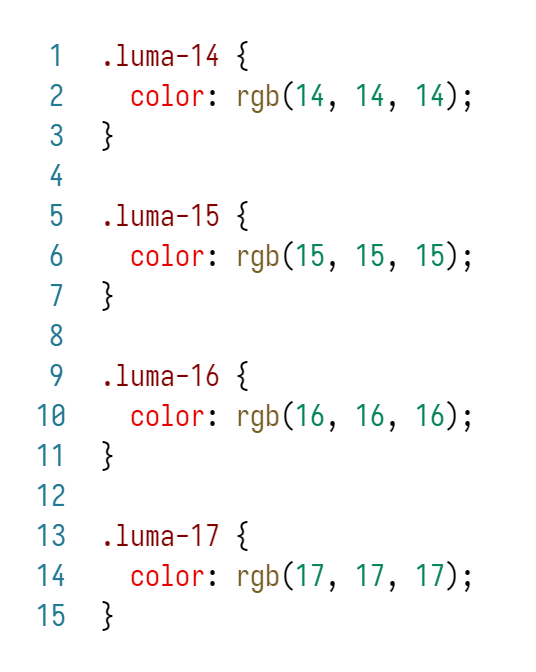
\includegraphics[width=\linewidth/\real{2.5}]{images/code-css-luma.png}
  \caption{Wycinek pliku \texttt{extra.css}, definiujący parę wariantów jednej z klas. Podobny kod jest powtórzony wiele razy w reszcie pliku.}
  \label{fig:css-css-luma}
\end{figure}

Szybkość wczytywania tego kodu jest poprawiana przez jego podatność na zmniejszenie rozmiaru poprzez bezstratną kompresję danych. Zawarty w używanej przez format \texttt{gzip} algorytm kompresji \texttt{DEFLATE} dużą część uwagi poświęca na usuwanie powtórzeń. Oznacza to, że dla kodu w powyższym rysunku, segmenty jak \texttt{".luma-"} czy \texttt{"\{ color: rgb ("} po pierwszym wystąpieniu były by zastępowane odniesieniami do wcześniejszych danych. Mimo to, same parametryzowane fragmenty mogą zabrać niemałą ilość czasu i transferu danych.

Mechanizmem, który niweluje konieczności takiego powtarzania, to funkcjonalność o nazwie \texttt{Custom Properties}\footnote{\url{https://www.w3.org/TR/css-variables/}}, zwana także jako \texttt{CSS}'owe zmienne. Pozwalają nam one napisać kod \texttt{CSS}, który może wykorzystywać definiowane przez nas parametry, i używać ich do obliczeń wbudowanych właściwości \texttt{CSS}.

Żeby stworzyć taką zmienną, można użyć podobnej składni, co przy deklarowaniu normalnych właściwości, lecz nadając wybraną nazwę poprzedzoną dwoma myślnikami, np. \texttt{"-\.-columns: 10;"}. Żeby użyć zmiennej w deklaracji innej właściwości, należy użyć \texttt{CSS}'owej funkcji \texttt{var}, podając jej nazwę zmiennej, oraz opcjonalnie, po przecinku, domyślą wartość, np. \texttt{"color: var(-\.-main-text-color, black);"}.

Można więc zastąpić wszystkie parametryzowane klasy \texttt{luma-\#} oraz \texttt{luma-bg-\#} dwoma nieparametryzowanymi, ale korzystających ze zmiennych:

\begin{figure}[H]
  \centering
  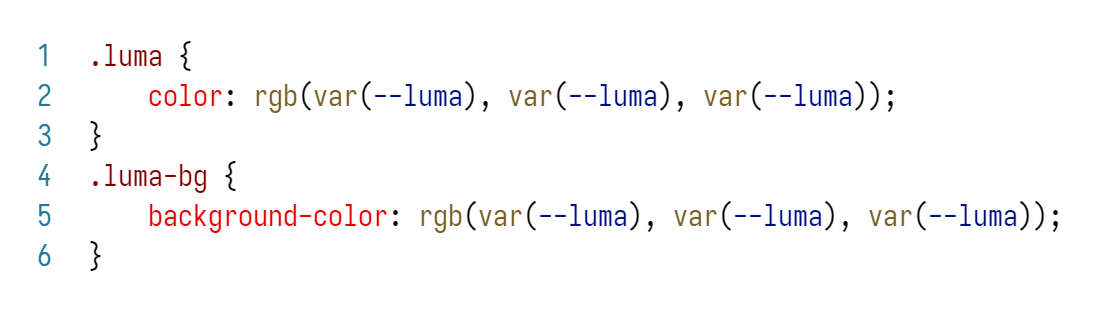
\includegraphics[width=\linewidth]{images/code-css-luma-vars.png}
  \caption{Klasy \texttt{luma} i \texttt{luma-bg}, używające zmiennych \texttt{CSS}}
  \label{fig:css-css-luma-vars}
\end{figure}

Konsekwencją przerzucenia się na taki model jest to, że co wcześniej było ustawieniem jednej klasy, teraz wymaga ustawienia klasy oraz parametru\footnote{Istnieją możliwości pominięcia tworzenia klasy, używając faktu, że błędne właściwości, np. przez korzystanie z niezdefiniowanych zmiennych, są ignorowane, lub poprzez przeszukiwanie własności \texttt{style} na elemencie html. Sposoby te mają niestety swoje wady.}. Tak więc w użyciu, atrybuty na elemencie zmieniają się z \texttt{class="luma-100"} na \texttt{class="luma" style="-\.-luma: 100;"}.

Trzecia z klas w tej samej grupie, \texttt{fix-text}, wymaga większej złożoności w implementacji zamiennika korzystającego ze zmiennych \texttt{CSS}. Ponieważ przetwarzanie zmiennych wewnątrz \texttt{CSS}'u jest bardzo ograniczone, nawet trywialne w innych językach zadania, jak potrzebne tutaj warunkowe wybranie jednej z dwóch wartości, wymaga użycia sztuczek i niekonwencjonalnych technik.

Do przetwarzania parametrów wewnątrz kodu \texttt{CSS} używa się funkcji \texttt{calc}\footnote{\url{https://drafts.csswg.org/css-values/\#calc-func}}. Można wewnątrz niej dokonywać operacji na danych, lecz zakres operacji, które możemy przeprowadzić, jest znacznie ograniczony. Dostępne jest dodawanie, odejmowanie, mnożenie i dzielenie, oraz funkcje \texttt{min}, \texttt{max} i \texttt{clamp}\footnote{\texttt{clamp} łączy funkcje \texttt{min} oraz \texttt{max}, obliczając \texttt{clamp(MIN, VAL, MAX) = max(MIN, max(VAL, MAX))}}. W nowszych przeglądarkach jest też dostęp do funkcji trygonometrycznych, oraz trwają pracę nad ustandaryzowaniem funkcji wykładniczych, logarytmicznych i zaokrąglających.

Pomimo tych ograniczeń, jest możliwe zareplikować wymaganą funkcjonalność. Można użyć funkcji generujących kolor, w tym przypadku \texttt{hsl}\footnote{\url{https://drafts.csswg.org/css-color/\#the-hsl-notation}}, aby wygenerować kolory o zdanej światłości. Ponieważ światłość w modelu opisu koloru \texttt{HSL} jest wartością od $0\%$ do $100\%$, wszystkie wartości poniżej $0\%$ będą traktowane jak $0\%$, natomiast wszystko powyżej $100\%$ jako $100\%$. Jeżeli więc stworzona zostanie funkcja, która będzie generowała wartości $\leq 0$ dla wartości parametru \texttt{-\.-luma}, dla której kolorem tekstu ma być czarny, oraz wartości $> 0$ kiedy kolor ten ma być biały, możemy przekazać tą wartość to funkcji koloru \texttt{hsl} po pomnożeniu przez dużą liczbę.

\begin{figure}[H]
  \centering
  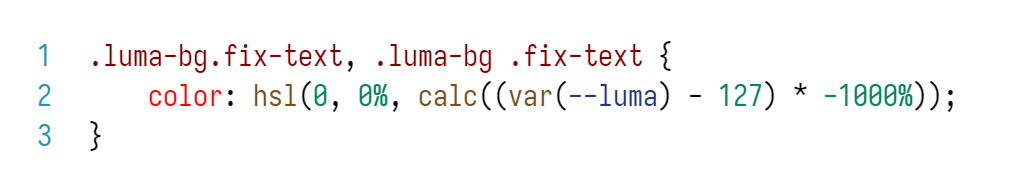
\includegraphics[width=\linewidth]{images/code-css-luma-calc.png}
  \caption{Klasa \texttt{CSS} dokonująca obliczeń, aby wybrać pasujący kolor}
  \label{fig:css-css-luma-calc}
\end{figure}

Możemy przeanalizować, jak powyższy kod działa, wykonując obliczenia w bloku \texttt{calc}, pamiętając o ograniczeniu zakresu liczbowego funkcji \texttt{hsl}. Gdyby \texttt{var(-\.-luma)} była równa $100$, to obliczono by
\[
  \left(100-127\right) \times -1000\% = -27 \times -1000\% = 27000\%
\]
\[
  \min\left(100\%, \max\left(0\%, 27000\%\right)\right) = \min\left(100\%, 27000\%\right) = 100\%
\]
Tak więc dla parametru \texttt{-\.-luma} równemu $100$, otrzymano kolor \texttt{hsl(0, 0\%, 100\%)}, czyli biały. Wstawiając zamiast $100$ w to samo równanie $128$, czyli wartość, dla której powinien zostać wygenerowany kolor czarny, otrzymano

\[
  \left(128-127\right) \times -1000\% = 1 \times -1000\% = -1000\%
\]
\[
  \min\left(100\%, \max\left(0\%, -1000\%\right)\right) = \min\left(100\%, 0\%\right) = 0\%
\]

Można wiec zauważyć, że dla wartości parametru powyżej $127$, wynikiem obliczenia będzie kolor o jasności $100\%$, natomiast poniżej o jasności $0\%$. Dla niecałkowitych własności parametru \texttt{-\.-luma} ta formuła nie zawsze działa. Np. dla \texttt{-\.-luma} równego $126.95$ obliczenia dają $\left(126.95-127\right)\times-1000\% = -0.05 \times -1000\% = 50\%$, co na stronie wyświetli kolor szary. Można zmniejszyć, jaki duży jest obszar dookoła punktu zmiany między białym a czarny, w którym formuła nie działa poprawnie, zwiększając procentowy mnożnik. Dla $1000\%$, wartości mniejsze od punktu zmiany o mniej niż $0.1$ będą miały to niepożądane zachowanie, gdyż $1000\%\times0.1 = 100\%$. Gdybyśmy chcieli, aby ta akceptowalna różnica od granicy była równa $0.05$, możemy policzyć $\frac{100\%}{0.05} = 2000\%$, co byłoby wartością dla ujemnego mnożnika w formule dla wersji w takim marginesem precyzji.

Można więc zastąpić wcześniejsze wersje klas \texttt{luma-\#} za pomocą następujących trzech deklaracji \texttt{CSS}:

\begin{figure}[H]
  \centering
  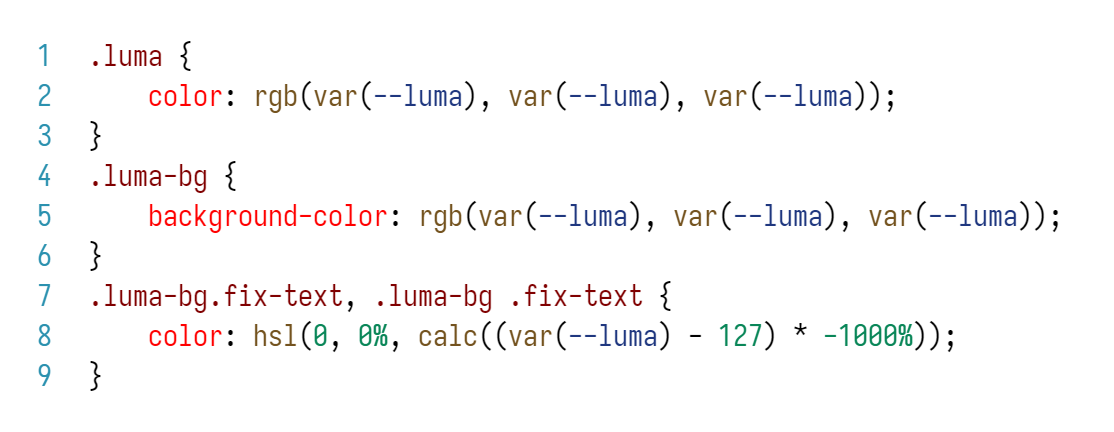
\includegraphics[width=\linewidth]{images/code-css-luma-all.png}
  \caption{Kod \texttt{CSS} zastępujący funkcjonalność klas pomocniczych z pliku \texttt{extra.css}, które ustawiały kolory obiektu na zadany odcień szarości}
  \label{fig:css-css-luma-all}
\end{figure}

Prócz tego potrzene jest dostosowanie kodu generującego elementy do tych zmian. Jeżeli są one tworzone za pomocą bezpośrednich API przeglądarki, zmiana ta jest prosta. Korzystanie z bibliotek ułatwiających tworzenie interfejsów nie powinno sprawić, że zmiana taka byłaby złożona.

\begin{figure}[H]
  \centering
  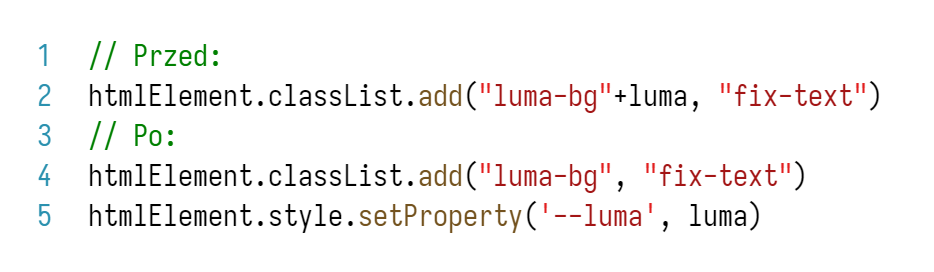
\includegraphics[width=\linewidth]{images/code-js-luma-adjust.png}
  \caption{Zmiana w kodzie \texttt{JavaScript}, który generował elementy korzystające z klas pomocniczych \texttt{luma-\dots}}
  \label{fig:code-js-luma-adjust}
\end{figure}

Kontynuując zamienianie klas pomocniczych na klasy wykorzystujące zmienne \texttt{CSS}, zastąpiono dwie klasy działające wspólnie, \texttt{col-\#} oraz \texttt{row-\#}. Ich działanie polega na stworzeniu siatki w szachownicę, gdzie kolory elementów tej siatki zmieniają się w taki sposób, że elementy po skosie mają ten sam kolor, a elementy ortogonalnie przyległe różnią się nim.

\begin{figure}[H]
  \centering
  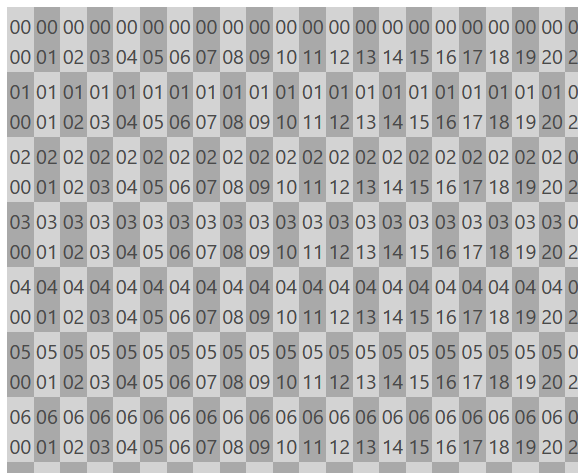
\includegraphics[width=\linewidth/\real{1.5}]{images/ui-grid-darken.png}
  \caption{Pożądany efekt}
  \label{fig:ui-grid-darken}
\end{figure}

Do zastąpienia tych klas można skorzystać z \texttt{CSS}'owej pseudoklasy \texttt{:nth-child()}. Jest ona uniwersalnie wspierana\footnote{\url{https://caniuse.com/mdn-css_selectors_nth-child}}, i pozwala na wybieranie elementów po ich kolejności na bazie formuły matematycznej. Ponieważ siatka na stronie składa się z elementu zawierającego wiersze, które to zawierają komórki, można prosto naprzemiennie pokolorować parzyste i nieparzyste wiersze.

\begin{figure}[H]
  \centering
  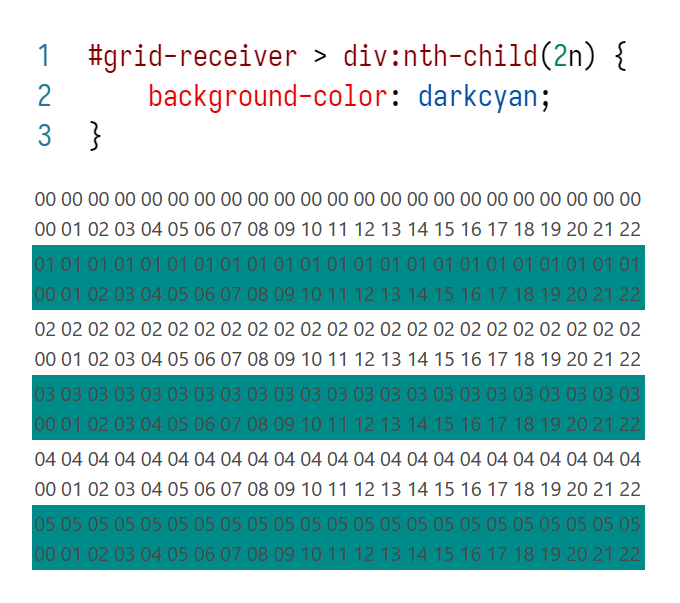
\includegraphics[width=\linewidth/\real{1.6}]{images/codeui-row-coloring.png}
  \caption{Fragment kodu oraz efekt, jaki ma on na siatkę. Warto zwrócić uwagę, że liczenie kolejności elementu zaczyna się od $1$, nie od $0$, więc wiersze pod nieparzystymi indeksami według kodu JavaScript są parzyste według \texttt{CSS}}
  \label{fig:codeui-row-coloring}
\end{figure}

Można więc wybrać dla tych wierszy tylko ich parzyste komórki, oraz dodać kod wybierające nieparzyste komórki nieparzystych wierszy.

\begin{figure}[H]
  \centering
  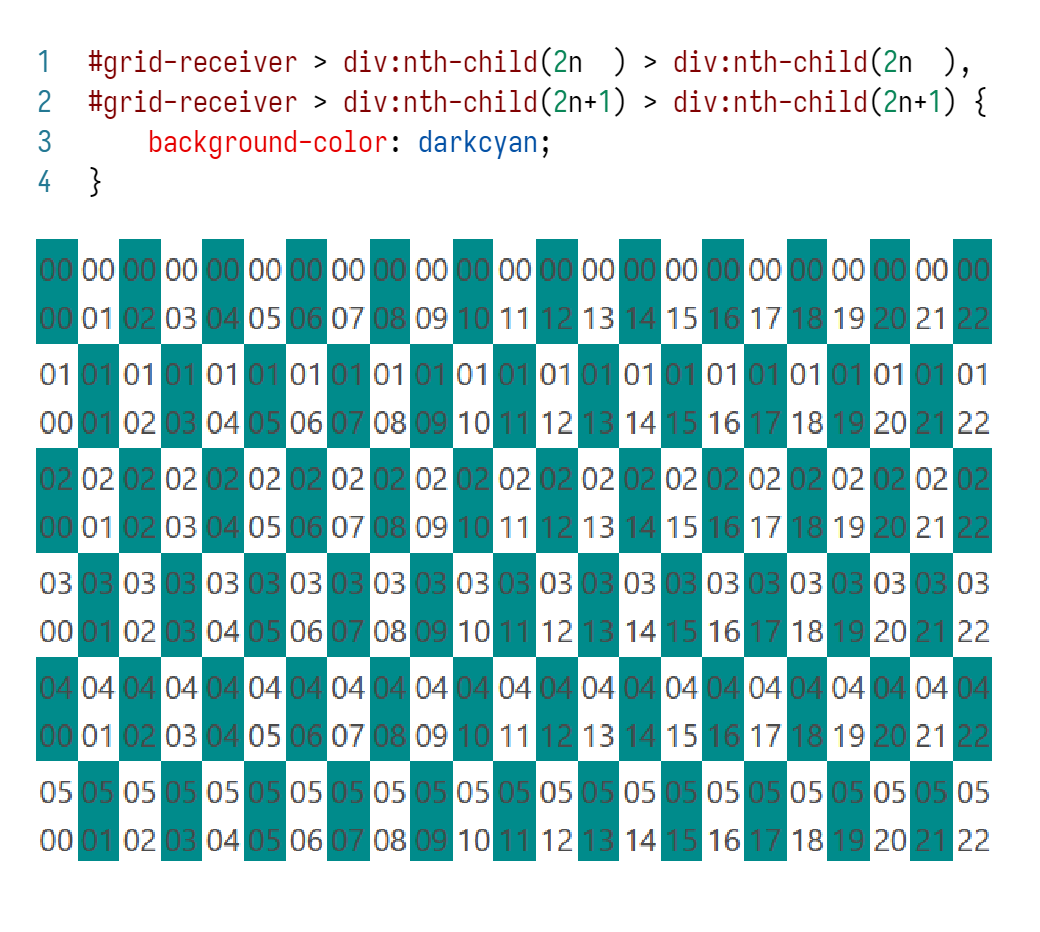
\includegraphics[width=\linewidth/\real{1.6}]{images/codeui-checkerboard-half-coloring.png}
  \caption{Stylowanie połowy szachownicy w siatce}
  \label{fig:codeui-checkerboard-half-coloring}
\end{figure}

Pozostaje dodać kod do przeciwnych wypadków, czyli parzystych komórek nieparzystych wierszy oraz nieparzystych komórek parzystych wierszy.

\begin{figure}[H]
  \centering
  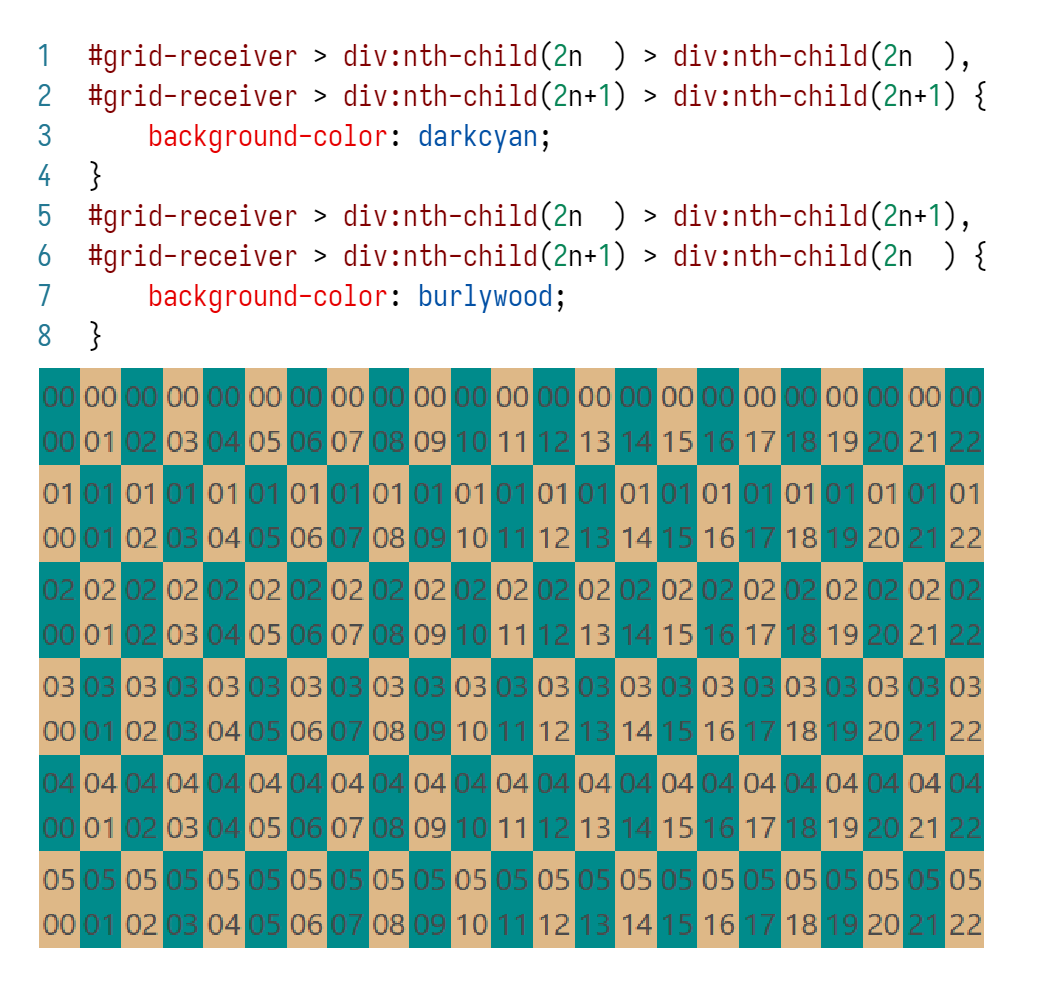
\includegraphics[width=\linewidth/\real{1.6}]{images/codeui-checkerboard-coloring.png}
  \caption{Stylizowanie całości szachownicy}
  \label{fig:codeui-checkerboard-coloring}
\end{figure}

Do pełnego pożądanego efektu pozostaje wybrać kolory dla danych części szachownicy. Niestety, taki sposób ma problem, nad rozwiązaniem którego są aktywnie prowadzone prace\footnote{\url{https://drafts.csswg.org/selectors/\#example-3c07f717}}, a jest nim to, że nie możemy wykluczyć elementów z bycia uwzględnianymi w liczeniu parzystości. Oznacza to, że gdyby mieć w takiej siatce wiersze niebędące częścią szachownicy, np. separatory między różnymi przedstawianymi zbiorami, zaburzałyby one dopasowania do formuły parzystości. Od niedawna dostępna jest opcja dodania selektora \texttt{CSS}, który określa, które z elementów mają być uwzględniane do liczenia tej formuły, i choć funkcja ta jest szeroko wspierana\footnote{\url{https://caniuse.com/css-nth-child-of}}, jest dalej nowa, a jej standaryzacja niezakończona.

Kolejnym elementem optymalizacji \texttt{CSS} który można wykonać jest wycięcie z biblioteki \texttt{Bulma} tylko tych części, które są potrzebne do funkcjonowania strony. Bulma wspiera proste tworzenie zmodyfikowanych jej wersji poprzez skorzystanie z języka \texttt{Scss}, który jest rozszerzeniem \texttt{CSS}. Można więc zaimportować tylko części biblioteki, które są potrzebne, i skompilować je do pliku \texttt{CSS}.

\begin{figure}[H]
  \centering
  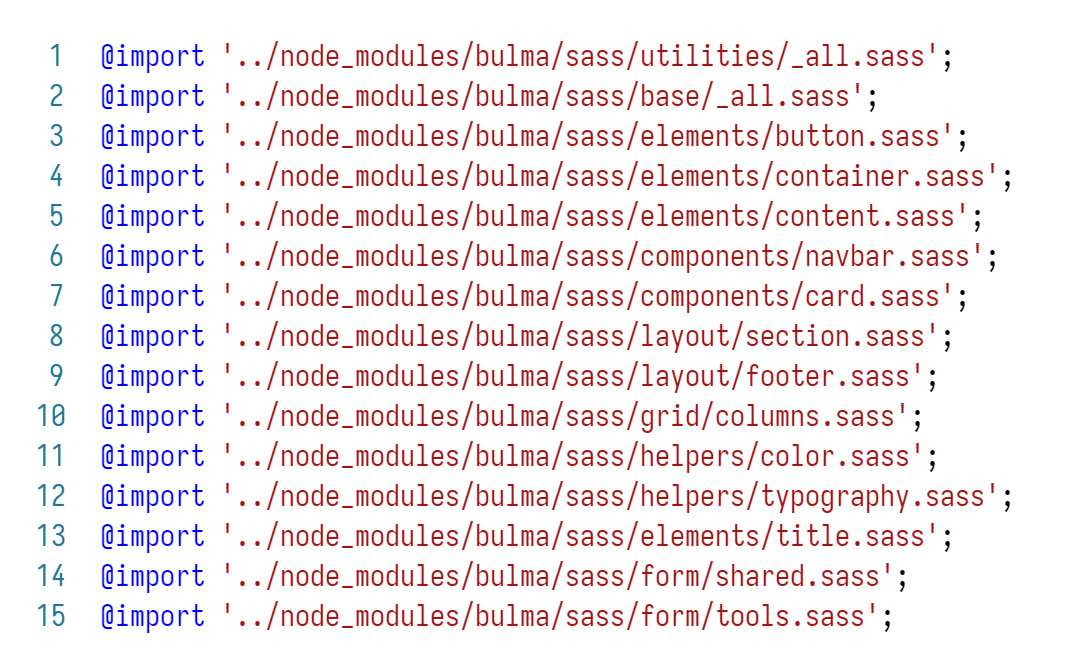
\includegraphics[width=\linewidth/\real{1.5}]{images/code-scss-import-bulma.png}
  \caption{Plik \texttt{Scss} importujący fragmenty biblioteki Bulma, wybierając tylko używane na stronie jej elementy}
  \label{fig:code-scss-import-bulma}
\end{figure}

Ponieważ w ramach projektu budowane są pliki biblioteki, oraz ponieważ plik \texttt{extra.css} stał się po zoptymalizowaniu bardzo mały, można połączyć je w jeden plik, który będzie spełniał funkcję ich obu. Takie połączenie pomaga ze stałym kosztem przesyłania danych drzewa Huffmana na początku skompresowanych \texttt{gzip}'em plików.

Na końcu można dokonać minifikacji generowanych plików \texttt{CSS}. Minifikacja polega na usunięciu pomocnych dla czytelności białych znaków z miejsc, gdzie nie mają one znaczenia dla treści \texttt{CSS}'owych definicji. Można do tego użyć narzędzi jak \href{https://www.npmjs.com/package/uglifycss}{uglifycss}, które można użyć z wiersza polecenia lub skryptu \texttt{JavaScript}.

Wykonując na tak zoptymalizowanym kodzie test WebPageTest'u, otrzymano następujące wyniki:

\begin{figure}[H]
  \centering
  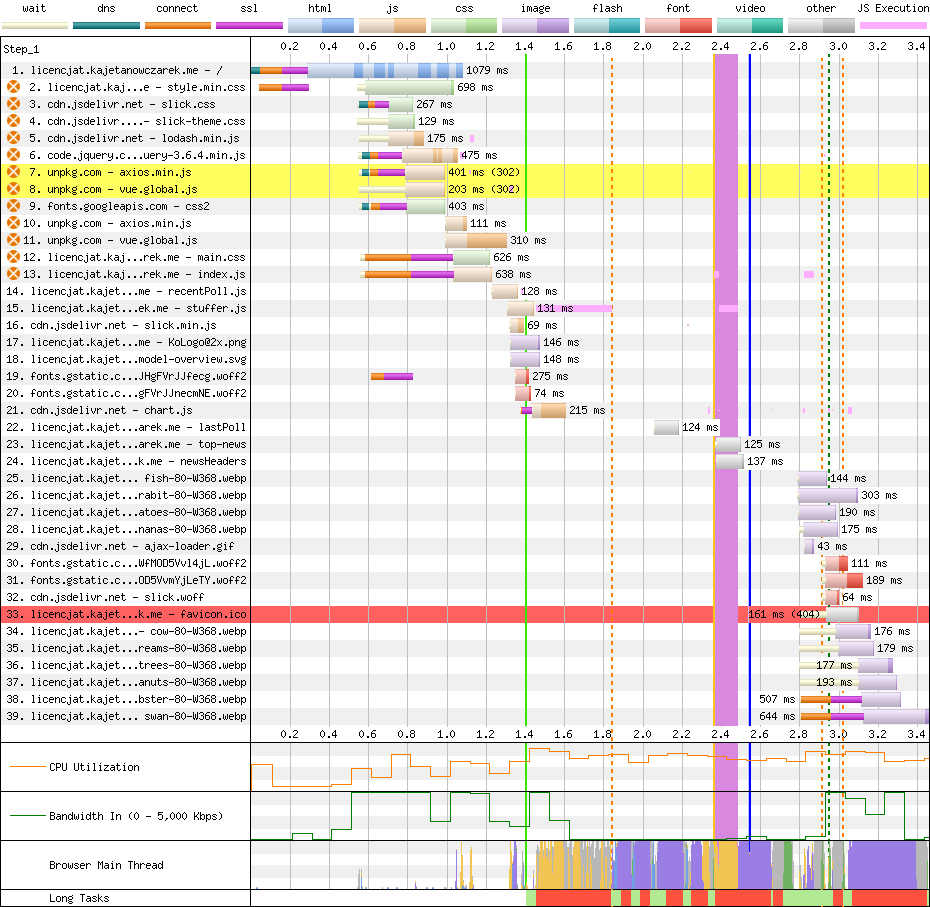
\includegraphics[width=\linewidth]{images/waterfall-after-css.png}
  \caption{Wyniki po poprawieniu plików \texttt{CSS}}
  \label{fig:waterfall-after-css}
\end{figure}

Porównując z poprzednimi wynikami, to choć witryna wczytuje się łącznie nieco dłużej, o około $0.1s$, tak rozpoczęcie renderowania ma miejsce około $0.2s$ wcześniej. Oznacza to, że użytkownicy wcześniej dostają jakąś treść na ekranie, ale po tych specyficznych zmianach musimy poczekać nieco dłużej na pełne wczytanie się zdjęć. Mimo to, szybsze wyświetlenie zawartości strony jest warte dla doświadczenia użytkowników witryny więcej, niż przyśpieszenie momentu jej pełnej gotowości.

\section{Wczytywanie treści HTML asynchronicznie}

Elementem powstrzymującym witrynę przed byciem widoczną i używalną jest duży i wolno wczytujący się główny plik \texttt{html}. Jego rozmiar wynika z tego, że zawiera on bardzo dużą ilość treści, przez co strona jest bardzo długa, i znaczna część jej prezentowalnej zawartości jest daleko poza wstępnym widokiem. Można opóźnić wczytywanie tej treści do po tym, jak wczyta się pierwszy widok na stronie.

Metodą, której można użyć do wczytywania treści \texttt{html} w sposób szybki i wydajny, to użycie możliwości strumieniowania danych połączeń tworzonych przez funkcję \texttt{fetch} oraz tworzenie dodatkowych instancji dokumentów html w ramach jednego okna przeglądarki.

Podstawowym konceptem, który wykorzystuje ta technika, to tworzenie nowych, częściowych dokumentów przy użyciu funkcji \texttt{document.implementation.createHTMLDocument}. Pozwala ona stworzyć dokument przeglądarki, który nie jest powiązany z żadnym oknem lub kontekstem renderowania, więc podczas dodawania do niego treści nie będą dokonywane obliczenia układu strony lub wczytywanie treści wizualnych. Używając \texttt{document.write} na stworzonym w taki sposób dokumencie można wstawiać w niego nowy kod \texttt{html} w trakcie, gdy jest on pobierany.

Aby nałożyć na siebie pobieranie, dekodowanie i interpretowanie danych, należy użyć systemu strumieni. Używając funkcji \texttt{fetch}, aby pobrać dane z serwera, po nawiązaniu połączenia można użyć właściwości \texttt{body} na obiekcie odpowiedzi, aby uzyskać dostęp do strumienia przychodzących danych. Strumień ten składa się z niezinterpretowanych bajtów, które potrzeba przekonwertować na tekst przy użyciu danego kodowania. Taką operację wykonują obiekty klasy \texttt{TextDecoderStream}, na którego strumień wejścia można wysyłać sekwencje bajtów, a on na swoim strumieniu wyjścia będzie emitował kolejne \texttt{string}'i. 

Łącząc te koncepty w całość, otrzymano następujący kod:

\begin{figure}[H]
  \centering
  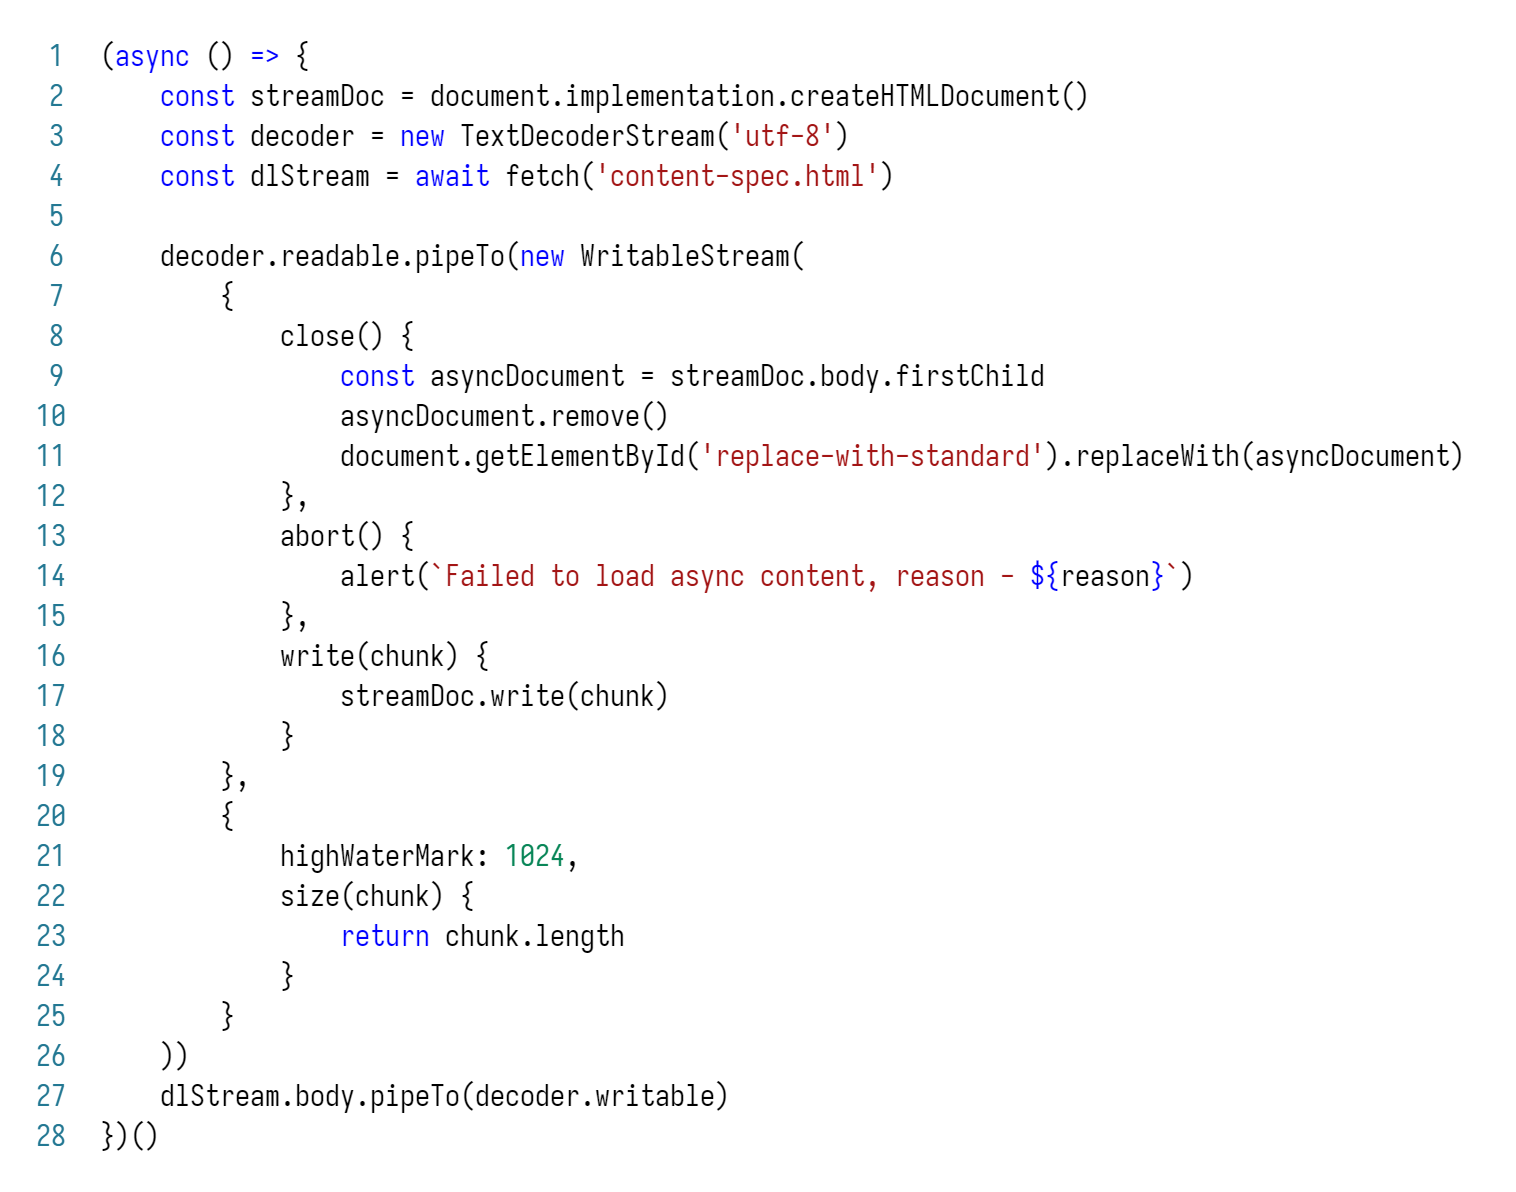
\includegraphics[width=\linewidth]{images/code-js-async-streaming.png}
  \caption{Kod wczytujący zasób \texttt{content-spec.html} w sposób asynchroniczny, a następnie wstawiający wczytaną zawartość do treści witryny. W celu połączenia ze sobą strumieni, używana jest metoda \texttt{pipeTo}. Celem odebrania treści ze strumienia dekodera, stworzono \texttt{WritableStream}, który po otrzymaniu fragmentu kodu w metodzie \texttt{write} wpisuje je do oddzielnego dokumentu, a po zamknięciu w metodzie \texttt{close} przemieszcza wczytaną zawartość między dokumentami.}
  \label{fig:code-js-async-streaming}
\end{figure}

Dodając ten kod do strony, i zastępując treści z pliku \texttt{index.html}, która teraz będzie wczytywana, elementem o \texttt{id} \texttt{replace-with-standard}, a następnie testując wydajność witryny po zmianach, otrzymano następujące wyniki:

\begin{figure}[H]
  \centering
  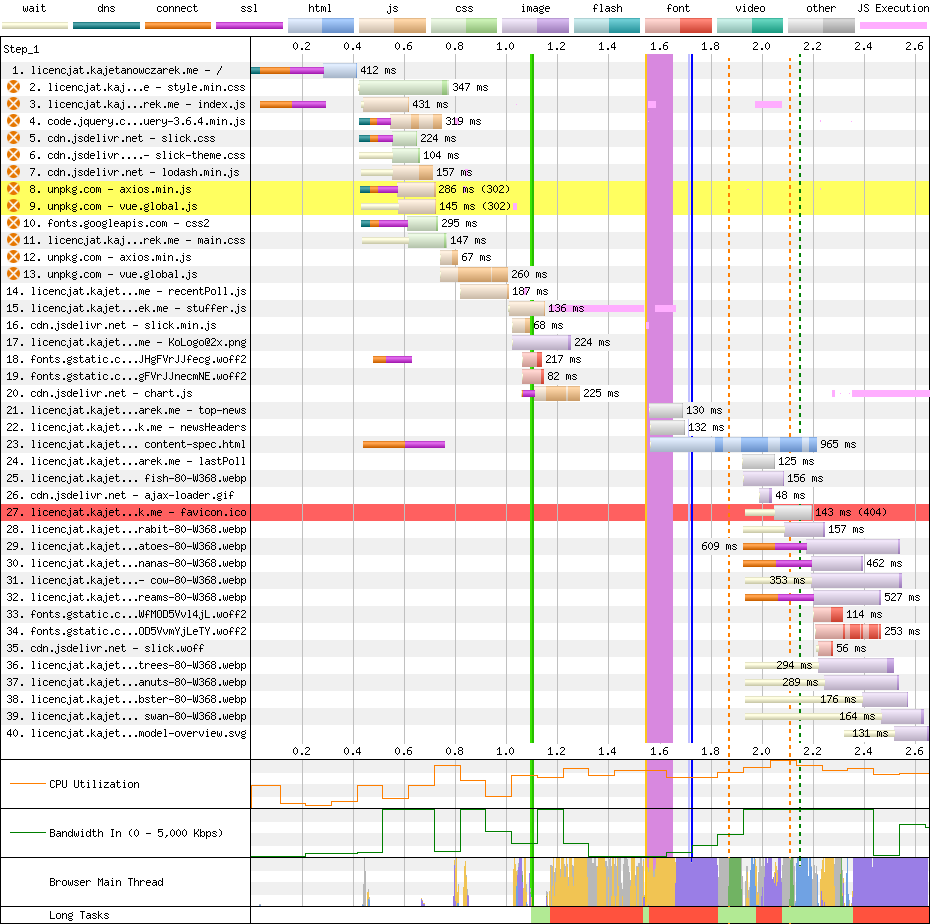
\includegraphics[width=\linewidth]{images/waterfall-after-async-html.png}
  \caption{Wyniki pomiarów po wdrożeniu asynchronicznego wczytywanie dużych treści \texttt{html}}
  \label{fig:waterfall-after-async-html}
\end{figure}

Porównując te wyniki, otrzymano wielką poprawę łącznego czasu wczytywania oraz rozpoczęcia renderowania. Czas do pierwszej treści na ekranie spadł z $1.4s$ do $1.05s$, co jest poprawą o $25\%$, a łączny czas wczytywania witryny spadł z $3.4$ do $2.6$ sekund. Zyskano więc znacznie na obu rodzajach szybkości wczytywania.

\section{Redukcja kodu JavaScript}

W projekcie wykorzystywane są dwie biblioteki JavaScript - \texttt{Vue} oraz \texttt{axios}. \texttt{Vue} służył to generowania elementów na stronie, których układ i struktura jest opisana w ramach wzorca tej biblioteki. Choć \texttt{Vue} jest praktycznym systemem, zezwalającym na proste tworzenie interaktywnych witryn, tak posiada o wiele więcej funkcji, niż jest potrzebne w ramach tego projektu, jak wsparcie animacji przejść, dynamicznej zmiany treści czy tworzenie nawigacji w ramach jednej stony. Prócz tego, użyta została wersja deweloperska biblioteki, a nie o wiele lepiej zoptymalizowanej i mniejsza wersja produkcyjna. Błędy takie są proste do zrobienia, gdy nie korzysta się ze współczesnych narzędzi do budowania stron, jak \texttt{vite} czy \texttt{webpack}, gdyż wymagane jest ręczne zarządzanie złożoności różnic między środowiskiem programisty a użytkownika. 

Ponieważ użyto \texttt{Vue} tylko do stworzenia stałej treści, można prosto zastąpić je niekorzystającym z tej biblioteki kodem \texttt{JavaScript}. W wersji korzystającej z \texttt{Vue}, definiowano wzorzec struktury kodu \texttt{HTML} zawartości, jaka ma zostać wstawiona na stronę, w formie tekstu, a biblioteka była odpowiedzialna za stworzenie z formy tekstowej i danych rzeczywistych elementów na stronie. Pozbywając się więc biblioteki, trzeba samemu tworzyć te elementy.

W tworzeniu elementów \texttt{HTML} przy użyciu surowego \texttt{JavaScript}'u można wyróżnić dwa podstawowe sposoby na tworzenie złożonych elementów. Pierwszy z nich, to przez modyfikowanie kodu \texttt{HTML} elementów za pomocą właściwości \texttt{innerHTML}, ustawiając ją na tekst zawierający docelowy kod. Drugi, to tworzenie elementów przy pomocy \texttt{document.createElement}, modyfikowanie ich, a potem umieszczanie w drzewie elementów dokumentu. Głównymi wadami pierwszej metody to suboptymalna wydajność, gdyż tworząc wiele elementów wiele razy uruchamiany jest parser \texttt{HTML}. Druga natomiast jest wielce niepraktyczna - ponieważ dostępne metody do tworzenia i manipulacji elementów \texttt{DOM} nie były oryginalnie designowane dla języka \texttt{JavaScript}\footnote{ISBN: 9780764588204, 21.1.}, są one względnie prymitywne, celem funkcjonowania w wielu różnych językach

W ramach tego projektu użyto hybrydowego rozwiązania, w ramach którego tworzone są oddzielne elementy \texttt{HTML} dla logicznych elementów prezentacji, ale struktura wysokopoziomowych elementów jest tworzona przy pomocy ustawiania własności \texttt{innerHTML}.

\begin{figure}[H]
  \centering
  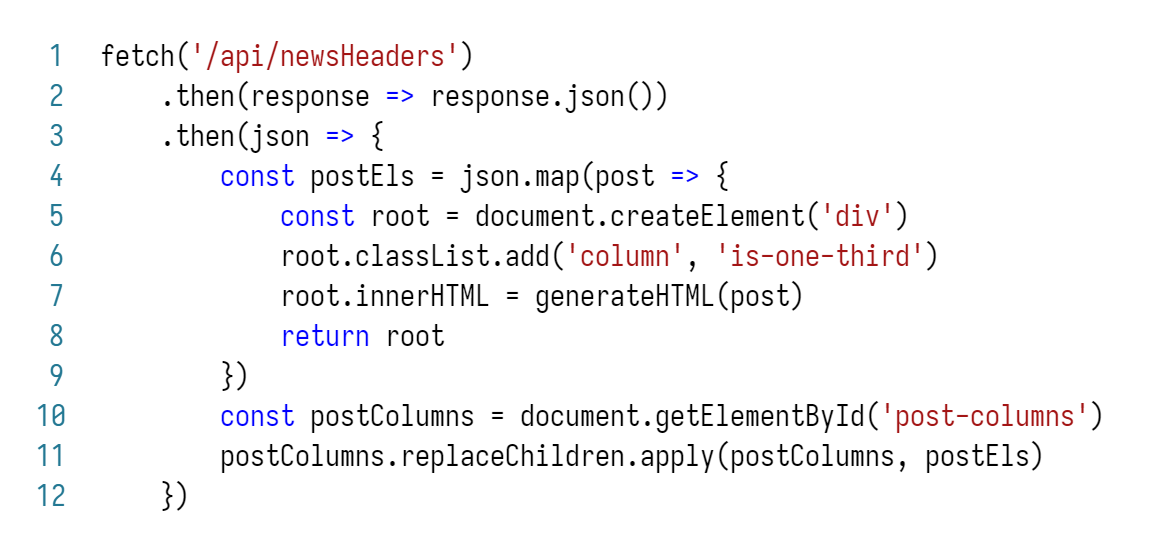
\includegraphics[width=\linewidth]{images/code-js-elem-gen.png}
  \caption{Kod \texttt{JavaScript} generujący siatkę postów. Po wczytaniu danych i przetworzeniu ich na używalny format, tworzony jest element \texttt{div}, ustawiamy na nim odpowiednie klasy, a następnie zmieniamy jego treść \texttt{HTML}.}
  \label{fig:code-js-elem-gen}
\end{figure}

Kolejną biblioteką, która może zostać usunięta, jest używany do pobierania danych z serwera \texttt{axios}. Stara się on ułatwić wykonywanie zapytań \texttt{HTTP} poprzez kod \texttt{JavaScript} witryny, lecz nie jest do tego niezbędny, oraz w przypadku testowej strony niewiele tego ułatwienia ma miejsce. Można do tego samego celu skorzystać z uniwersalnie wspieranej\footnote{\url{https://caniuse.com/fetch}} funkcji \texttt{fetch}, która oferuje praktyczny, prosty do użytku interfejs API, niezmiennie dysponując szerokimi możliwościami konfiguracji połączenia.

Dla projektu testowego, największą różnicą między tymi dwoma rozwiązaniami jest ich podejście do serializacji i deserializacji danych. \texttt{Axios} domyślnie konwertuje dane na obiekty \texttt{JavaScript}'owe, natomiast \texttt{fetch} wymaga, aby ręcznie rozpocząć tą konwersję.

\begin{figure}[H]
  \centering
  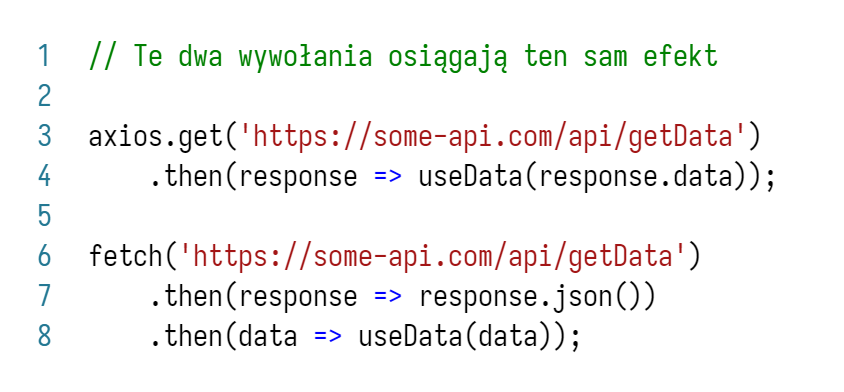
\includegraphics[width=\linewidth]{images/code-js-axios-v-fetch.png}
  \caption{Porównanie użycia biblioteki \texttt{axios} oraz wbudowanej w przeglądarkę funkcji \texttt{fetch}}
  \label{fig:code-js-axios-v-fetch}
\end{figure}

Można podmienić wykorzystania tych bibliotek kodem używającym interfejsy przeglądarki, a następnie wykluczyć je w pełni z kodu witryny, oszczędzając na ich przesyle danych. Po zastosowaniu takich zmian, i przetestowaniu ponownie strony, otrzymano następujące wyniki:

\begin{figure}[H]
  \centering
  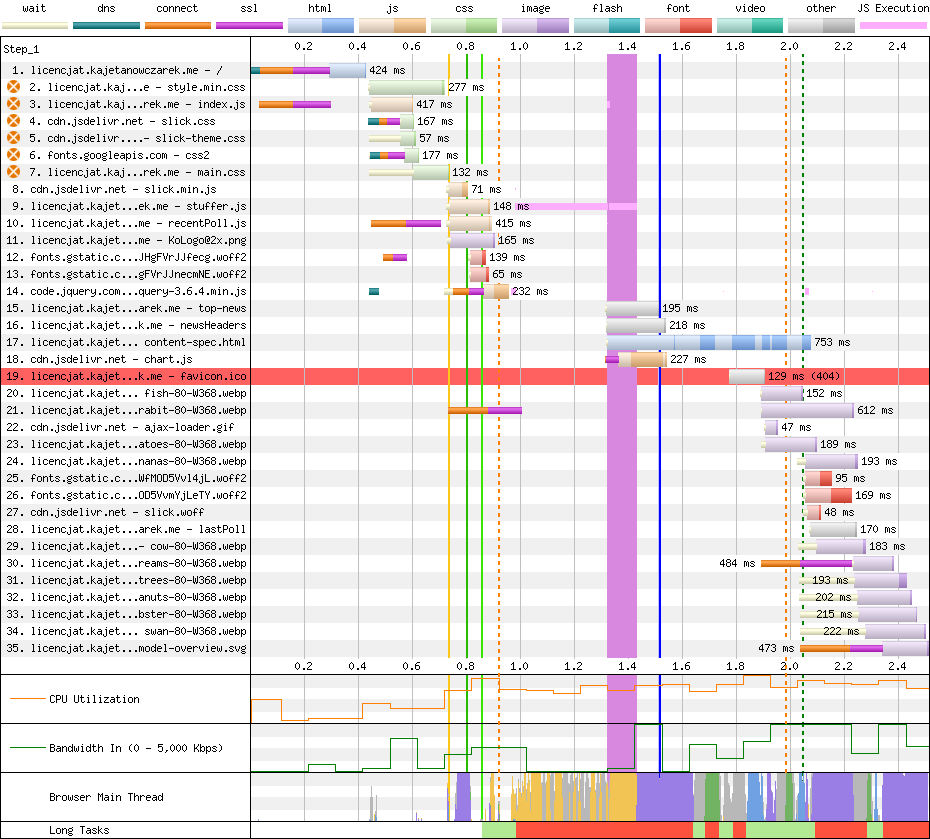
\includegraphics[width=\linewidth]{images/waterfall-after-jsreduction.png}
  \caption{Wyniki pomiarów po zastąpieniu bibliotek kodem specyficznym dla tego projektu.}
  \label{fig:waterfall-after-jsreduction}
  %https://www.webpagetest.org/customWaterfall.php?test=230717_BiDcB5_53K&run=3&width=930
\end{figure}

W porównaniu z poprzednimi wynikami, przyśpieszono łączny czas wczytywania witryny z $\approx2.6$s do $2.5$s, co jest niewielką poprawą. Pierwsze wyświetlenie treści natomiast zostało przesunięte o wiele wstecz, z $1.1$s do $0.8$s, co jest poprawą o ponad $25\%$.

\section{Optymalizacja wykonywania JavaScript}

Patrząc na poprzedni wykres, można zaobserwować przerwę w pobieraniu treści, podczas którego według legendy wykresu plik \texttt{stuffer.js} wykonuje kod \texttt{JavaScript}. Plik ten ma na celu stworzenie części strony, dokonując obliczeń i tworząc dynamicznie elementy, dodając je do treści zawartych w witrynie.

Podczas egzekucji tego kodu, były wykonywane wolne operacje, przede wszystkim użycie operatora \texttt{...}, który może być wykonywany dużą ilość czasu. Ponieważ operator ten wspiera \texttt{JavaScript}'owe iteratory, których ilość elementów może być nie znana, przetwarza on element po elemencie\footnote{\url{https://tc39.es/ecma262/multipage/ecmascript-language-expressions.html\#sec-runtime-semantics-arrayaccumulation}}, co przynajmniej w najpowszechniej używanej implementacji silnika \texttt{JavaScript}, czyli stworzone przez Google \texttt{V8}, powoduje wielokrotne kopiowanie danych podczas przemieszczania pamięci na skutek rozszerzania tablic.

Jeżeli danymi, na których miałby działać ten operator, są tablicami, można go zastąpić przy użyciu funkcji \texttt{apply}:
\begin{figure}[H]
  \centering
  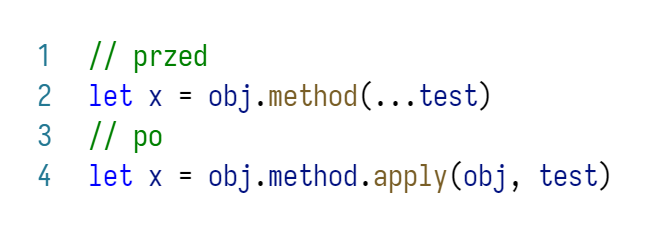
\includegraphics[width=\linewidth]{images/code-js-spread-operator.png}
  \caption{Sposób zastąpienia operatora \texttt{...} użyciem metody \texttt{apply}, obecnej na funkcjach}
  \label{fig:code-js-spread-operator}
\end{figure}

Temat optymalizacji kodu \texttt{JavaScript} jest niesłychanie złożony, gdyż większość logiki każdej poza prostymi stronami jest zawarta właśnie w tej części strony. Ponieważ projekt testowy jest względnie prosty, nie było w nim wiele okazji do zaprezentowania detali i technik przyśpieszania wykonywania tego języka. Pomimo tego, problem z używaniem operatora \texttt{...} jest powszechny i może znacznie wpłynąć na wydajność witryny.

Dokonując testów na wersji strony unikającej korzystania z operatora \texttt{...}, otrzymano następujące wyniki. 

\begin{figure}[H]
  \centering
  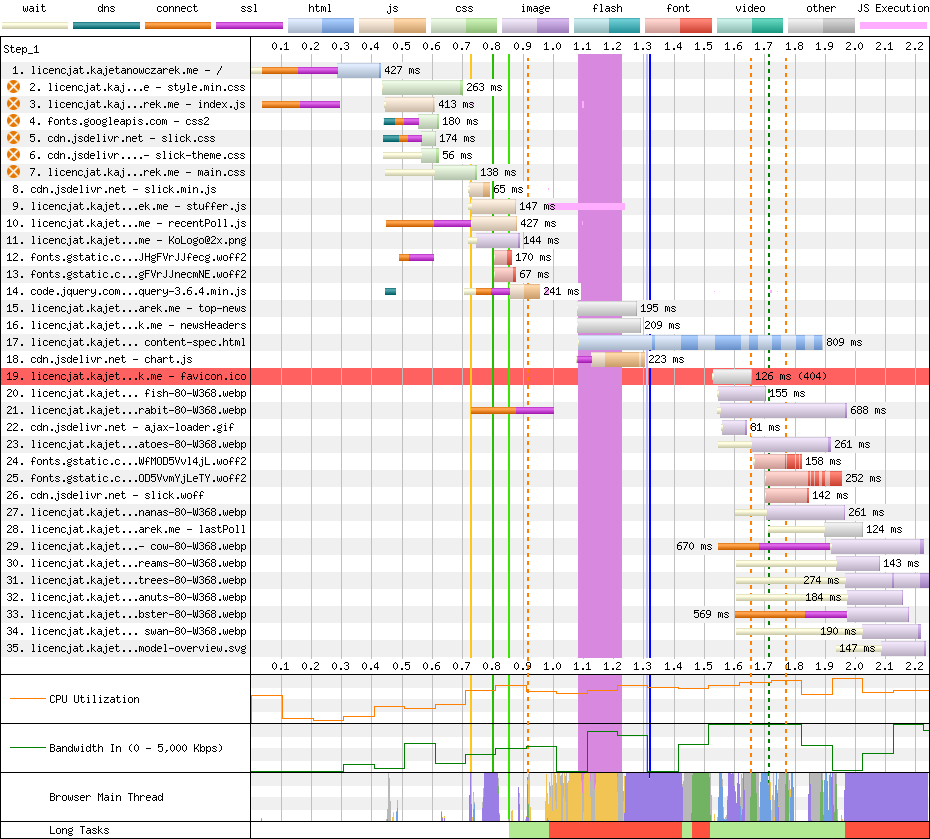
\includegraphics[width=\linewidth]{images/waterfall-after-no-array-spread.png}
  \caption{Wyniki pomiarów po zastąpieniu operatora \texttt{...} za pomocą metody funkcji \texttt{apply}}
  \label{fig:waterfall-after-no-array-spread}
  %https://www.webpagetest.org/result/230717_BiDcHT_5AC/1/details/#waterfall_view_step1
\end{figure}

W porównaniu z poprzednimi wynikami, czas potrzebny na pierwsze wyświetlenie zawartości na stronie nie uległ zmianie, gdyż wykonywanie zoptymalizowanego kodu miało miejsce po tym momencie. Ogólny czas wczytywania strony za to spadł z około $2.5$s do nieco ponad $2.2$s, dając około $10\%$ przyśpieszenia w ogólnym czasie wczytywania.

\chapter{Zakończenie}

\selfnote{JESZCZE NIE NAPISANE}

\begin{thebibliography}{7}
\addcontentsline{toc}{chapter}{Bibliografia}
%
\bibitem{Lang}
Serge Lang, 
\textit{Algebra. Revised third edition}, 
New York, Springer-Verlag, 2002.
%
\bibitem{Kostrykin} 
Aleksiej Kostrykin, 
\textit{Wstęp do algebry. Podstawy algebry},
Warszawa, Wydawnictwo Naukowe PWN, 2022.
\end{thebibliography}
\end{document}